\documentclass[11pt,a4paper]{article}
\usepackage[utf8]{inputenc}
\usepackage[margin=2.5cm]{geometry}
\usepackage{iohk}
\usepackage{microtype}
\usepackage{mathpazo} % nice fonts
\usepackage{amsmath}
\usepackage{amssymb}
\usepackage{latexsym}
\usepackage{mathtools}
\usepackage{stmaryrd}
\usepackage{extarrows}
\usepackage{slashed}
\usepackage[colon]{natbib}
\usepackage[unicode=true,pdftex,pdfa,colorlinks=true]{hyperref}
\usepackage{xcolor}
\usepackage[capitalise,noabbrev,nameinlink]{cleveref}
\usepackage{float}
\floatstyle{boxed}
\restylefloat{figure}
\usepackage{listings} % for code blocks.
%%
%% Package `semantic` can be used for writing inference rules.
%%
\usepackage{semantic}
%% Setup for the semantic package
\setpremisesspace{20pt}
\usepackage{tikz}
\usetikzlibrary{decorations.pathreplacing, positioning, arrows.meta, calc}
% For drawing simple diagrams involving arrows between LaTeX symbols
\usepackage{tikz-cd}

%%
%% Types
%%
\newcommand{\Bool}{\type{Bool}}
\newcommand{\Tx}{\type{Tx}}
\newcommand{\Ix}{\type{Ix}}
\newcommand{\TxId}{\type{TxId}}
\newcommand{\Addr}{\type{Addr}}
\newcommand{\UTxO}{\type{UTxO}}
\newcommand{\Value}{\type{Value}}
\newcommand{\Lovelace}{\type{Lovelace}}
\newcommand{\UTxOEnv}{\type{UTxOEnv}}
\newcommand{\UTxOState}{\type{UTxOState}}
%% Adding witnesses
\newcommand{\TxIn}{\type{TxIn}}
\newcommand{\TxOut}{\type{TxOut}}
\newcommand{\VKey}{\type{VKey}}
\newcommand{\SKey}{\type{SKey}}
\newcommand{\HashKey}{\type{HashKey}}
\newcommand{\SkVk}{\type{SkVk}}
\newcommand{\Sig}{\type{Sig}}
\newcommand{\Data}{\type{Data}}
%% Adding delegation
\newcommand{\Epoch}{\type{Epoch}}
\newcommand{\VKeyGen}{\type{VKey_G}}
%% Blockchain
\newcommand{\Gkeys}{\var{G_{keys}}}
\newcommand{\Block}{\type{Block}}
\newcommand{\CEEnv}{\type{CEEnv}}
\newcommand{\CEState}{\type{CEState}}
\newcommand{\BDEnv}{\type{BDEnv}}
\newcommand{\BDState}{\type{BDState}}
\newcommand{\Slot}{\type{Slot}}
\newcommand{\SlotCount}{\type{SlotCount}}

%%
%% Functions
%%
\newcommand{\txins}[1]{\fun{txins}~ \var{#1}}
\newcommand{\txid}[1]{\fun{txid}~ \var{#1}}
\newcommand{\txouts}[1]{\fun{txouts}~ \var{#1}}
\newcommand{\values}[1]{\fun{values}~ #1}
\newcommand{\balance}[1]{\fun{balance}~ \var{#1}}
%% UTxO witnesses
\newcommand{\inputs}[1]{\fun{inputs}~ \var{#1}}
\newcommand{\wits}[1]{\fun{wits}~ \var{#1}}
\newcommand{\verify}[3]{\fun{verify} ~ #1 ~ #2 ~ #3}
\newcommand{\sign}[2]{\fun{sign} ~ #1 ~ #2}
\newcommand{\serialised}[1]{\llbracket \var{#1} \rrbracket}
\newcommand{\addr}[1]{\fun{addr}~ \var{#1}}
\newcommand{\hash}[1]{\fun{hash}~ \var{#1}}
\newcommand{\txbody}[1]{\fun{txbody}~ \var{#1}}
\newcommand{\txfee}[1]{\fun{txfee}~ \var{#1}}
\newcommand{\minfee}[2]{\fun{minfee}~ \var{#1}~ \var{#2}}
% wildcard parameter
\newcommand{\wcard}[0]{\underline{\phantom{a}}}
%% Adding ledgers...
\newcommand{\utxo}[1]{\fun{utxo}~ #1}
%% Delegation
\newcommand{\delegatesName}{\fun{delegates}}
\newcommand{\delegates}[3]{\delegatesName~#1~#2~#3}
\newcommand{\dwho}[1]{\fun{dwho}~\var{#1}}
\newcommand{\depoch}[1]{\fun{depoch}~\var{#1}}
%% Delegation witnesses
\newcommand{\dbody}[1]{\fun{dbody}~\var{#1}}
\newcommand{\dwit}[1]{\fun{dwit}~\var{#1}}
%% Blockchain
\newcommand{\bwit}[1]{\fun{bwit}~\var{#1}}
\newcommand{\bslot}[1]{\fun{bslot}~\var{#1}}
\newcommand{\bbody}[1]{\fun{bbody}~\var{#1}}
\newcommand{\bdlgs}[1]{\fun{bdlgs}~\var{#1}}
%% Set notation
\newcommand\Set[2]{\{\,#1\mid#2\,\}}
%% Let bindings
\newcommand{\leteq}{\ensuremath{\mathrel{\mathop:}=}}

%% For properties
\newcommand{\txs}{\ensuremath{\mathcal{T}}}
\newcommand{\transtar}[2]{\xlongrightarrow[\textsc{#1}]{#2}\negthickspace^{*}}
\newcommand{\biguo}[1]{\ensuremath{\underset{#1}{\underrightarrow\bigcup}}}

%\includeonly{update-mechanism, delegation, blockchain-interface}

%% Parameters that control floats placement. See https://robjhyndman.com/hyndsight/latex-floats/
\setcounter{topnumber}{2}
\setcounter{bottomnumber}{2}
\setcounter{totalnumber}{4}
\renewcommand{\topfraction}{0.85}
\renewcommand{\bottomfraction}{0.85}
\renewcommand{\textfraction}{0.15}
\renewcommand{\floatpagefraction}{0.7}
\newcommand{\DEnv}{\type{DEnv}}
\newcommand{\DSEnv}{\type{DSEnv}}
\newcommand{\DSState}{\type{DSState}}
\newcommand{\DCert}{\type{DCert}}
\newcommand{\DState}{\type{DState}}
\newcommand{\DEState}{\type{DEState}}


\newtheorem{definition}{Definition}
\newtheorem{property}{Property}

\begin{document}

\hypersetup{
  pdftitle={A Formal Specification of the Cardano Ledger},
  breaklinks=true,
  bookmarks=true,
  colorlinks=false,
  linkcolor={blue},
  citecolor={blue},
  urlcolor={blue},
  linkbordercolor={white},
  citebordercolor={white},
  urlbordercolor={white}
}


  \cleardoublepage%
  \tableofcontents%
  \listoffigures%
  \clearpage%

  \begin{changelog}
        \change{2019/10/08}{Jared Corduan, Polina Vinogradova and Matthias G\"udemann}{FM (IOHK)}{Initial version (0.1).}
        \change{2019/10/08}{Kevin Hammond}{FM (IOHK)}{Added cover page.}
      \end{changelog}
      \clearpage%
\begin{landscape}
\floatstyle{plain}
\restylefloat{figure}
\begin{figure*}
\includegraphics[scale=0.65]{d8-depends.pdf}
\caption{Positioning of this Deliverable.}
\end{figure*}
\end{landscape}
\floatstyle{boxed}
\restylefloat{figure}
\cleardoublepage
% \begin{center}
%   \large{Executive Summary}
% \end{center}

% \noindent
% This document provides a formal specification of the Cardano ledger for use in the Shelley implementation.
% It is intended to form the basis for an executable specification that will be the basis of the initial
% release.
% \cleardoublepage
\renewcommand{\thepage}{\arabic{page}}
\setcounter{page}{1}

\title{A Formal Specification of the Cardano Ledger}

\author{Jared Corduan  \\ {\small \texttt{jared.corduan@iohk.io}} \\
   \and Polina Vinogradova \\ {\small \texttt{polina.vinogradova@iohk.io}} \\
   \and Matthias G\"udemann  \\ {\small \texttt{matthias.gudemann@iohk.io}}}

%\date{}

\maketitle

\begin{abstract}
This document provides a formal specification of the Cardano ledger for use in the upcoming Shelley implementation.
It is intended to underpin a Haskell executable specification that will be the basis of the initial
Shelley release, and represents a core design and quality assurance document.
It will be used to define properties and tests, and to provide the basis for strong formal assurance
using mathematical proof techniques.
The document defines the rules for extending the ledger with transactions
that will affect both UTxO and stake delegation.
Key properties that have been identified include ...
% This will serve as the specification for random generators of transactions
% which adhere to the rules presented here, and that will.
\end{abstract}

\section*{List of Contributors}
\label{acknowledgements}

Nicol\'as Arqueros,
Nicholas Clarke,
Duncan Coutts,
Ruslan Dudin,
Sebastien Guillemot,
Vincent Hanquez,
Ru Horlick,
Michael Hueschen,
Yun Lu,
Philipp Kant,
Jean-Christophe Mincke,
Damian Nadales,
Nicolas Di Prima.


\tableofcontents
\listoffigures

\section{Introduction}
\label{sec:introduction-shelley}

This document is a formal specification of the functionality of the ledger
on the blockchain. The blockchain layer of the
protocol and the interaction between the ledger and the blockchain
layer is presented in a separate document, see~\cite{shelley_consensus}. The details of the
background and the larger context
for the design decisions formalized in this document are presented
in~\cite{delegation_design}

In this work,
we present important properties any implementation of the ledger must have.
Specifically, we model the following aspects
of the functionality of the ledger on the blockchain:

\begin{description}
\item[Preservation of value] Every coin in the system is accounted for,
  and the total amount is unchanged by every transaction and epoch change.
  In particular, every coin is accounted for by one of the following categories:
  \begin{itemize}
    \item Circulation (UTxO)
    \item Deposit pot
    \item Fee pot
    \item Reserves (monetary expansion)
    \item Rewards (account addresses)
    \item Reward pot (undistributed)
    \item Treasury
  \end{itemize}
\item[Witnesses] Authentication of parts of the transaction data by means of
  cryptographic entities (such as signatures and private keys) contained in
  these transactions.
\item[Delegation] Validity of delegation certificates, which delegate
  block-signing rights.
\item[Stake] Staking rights associated to an address.
\end{description}

While the blockchain protocol is a reactive system driven by the arrival
of blocks causing updates to the ledger, the formal description is a collection
of rules which is a
static description of what a \textit{valid ledger} is. The specifics of the
semantics we use to define and apply
the rules we present in this document are explained in detail in
\cite{small_step_semantics}. A valid ledger state can only
reached by applying a sequence of inference rules, and any valid ledger state
is reachable by applying some sequence of these rules.

The structure of the rules we give here is such that their application is
deterministic. That is, given a specific initial state and relevant environmental
constants, there is no ambiguity
about which rule should be applied at any given time (i.e.~which state
transition is allowed take place). This is an important property which reflects
the reality of the implementation --- the blockchain evolves in a particular way
given some user activity and the passage of time, and its behaviour is
never unexpected.


\section{Notation}
\label{sec:notation-shelley}

The transition system is explained in \cite{small_step_semantics}.

\begin{description}
  \item[Powerset] Given a set $\type{X}$, $\powerset{\type{X}}$ is the set of all
    the subsets of $X$.
  \item[Sequences] Given a set $\type{X}$, $\seqof{\type{X}}$ is the set of
    sequences having elements taken from $\type{X}$. The empty sequence is
    denoted by $\epsilon$, and given a sequence $\Lambda$, $\Lambda; \type{x}$ is
    the sequence that results from appending $\type{x} \in \type{X}$ to
    $\Lambda$.
  \item[Functions] $A \to B$ denotes a \textbf{total function} from $A$ to $B$.
    Given a function $f$ we write $f~a$ for the application of $f$ to argument
    $a$.
  \item[Inverse Image] Given a function $f: A \to B$ and $b\in B$, we write
    $f^{-1}~b$ for the \textbf{inverse image} of $f$ at $b$, which is defined by
    $\{a \mid\ f a =  b\}$.
  \item[Maps and partial functions] $A \mapsto B$ denotes a \textbf{partial
    function} from $A$ to $B$, which can be seen as a map (dictionary) with
    keys in $A$ and values in $B$. Given a map $m \in A \mapsto B$, notation
    $a \mapsto b \in m$ is equivalent to $m~ a = b$.
  \item[Map Operations] Figure~\ref{fig:notation:nonstandard}
    describes some non-standard map operations.
  \item[Relations] A relation on $A\times B$ is a subset of $A\times B$.
    Both maps and functions can be thought of as relations.
    A function $f:A\to B$ is a relation consisting of pairs $(a, f(a))$ such that $a\in A$.
    A map $m: A\mapsto B$ is a relation consisting of pairs $(a, b)$ such that
    $a\mapsto b \in m$.
    Given a relation $R$ on $A\times B$, we define the inverse relation $R^{-1}$ to be
    all pairs $(b, a)$ such that $(a, b)\in R$. Similarly, given a function $f:A\to B$ we
    define inverse relation $f^{-1}$ to consist of all pairs $(f(a), a)$.
    Finally, given two relations $R\subseteq A\times B$ and $S\subseteq B\times C$,
    we define the compostion $R\circ S$ to be all pairs $(a, c)$ such that
    $(a, b)\in R$ and $(b, c)\in S$ for some $b\in B$.
  \item[Option type] An option type in type $A$ is denoted as $A^? = A + \Nothing$. The
    $A$ case corresponds to a case when there is a value of type $A$ and the $1$
    case corresponds to a case when there is no value.

\end{description}

In Figure~\ref{fig:notation:nonstandard}, we specify the notation we use in
the rest of the document.

\begin{figure}[htb]
  \begin{align*}
    \var{set} \restrictdom \var{map}
    & = \{ k \mapsto v \mid k \mapsto v \in \var{map}, ~ k \in \var{set} \}
    & \text{domain restriction}
    \\
    \var{set} \subtractdom \var{map}
    & = \{ k \mapsto v \mid k \mapsto v \in \var{map}, ~ k \notin \var{set} \}
    & \text{domain exclusion}
    \\
    \var{map} \restrictrange \var{set}
    & = \{ k \mapsto v \mid k \mapsto v \in \var{map}, ~ v \in \var{set} \}
    & \text{range restriction}
    \\
    \var{map} \subtractrange \var{set}
    & = \{ k \mapsto v \mid k \mapsto v \in \var{map}, ~ v \notin \var{set} \}
    & \text{range exclusion}
    \\
    A \triangle B
    & = (A \setminus B) \cup (B \setminus A)
    & \text{symmetric difference}
    \\
    M \unionoverrideRight N
    & = (\dom N \subtractdom M)\cup N
    & \text{union override right}
    \\
    M \unionoverrideLeft N
    & = M \cup (\dom M \subtractdom N)
    & \text{union override left}
    \\
    M \unionoverridePlus N
    & = (M \triangle N)
    \cup \{k\mapsto v_1+v_2\mid {k\mapsto v_1}\in M \land {k\mapsto v_2}\in N \}
    & \text{union override plus} \\
    & & \text{(for monoidal values)}\\
  \end{align*}
  \caption{Non-standard map operators}
  \label{fig:notation:nonstandard}
\end{figure}

\clearpage


\section{Cryptographic primitives}
\label{sec:crypto-primitives-shelley}

Figure~\ref{fig:crypto-defs-shelley} introduces the cryptographic abstractions used in
this document. we begin by listing the abstract types, which are meant to
represent the corresponding concepts in cryptography. Only the functionality
explicitly stated in the figures below is assumed to be within the scope of this paper.
That is, their exact
implementation remains open to interpretation and we do not rely on
any additional properties derived from the study or implementation of public key
cryptography outside this work. The types and rules we give here are needed in
order to guarantee certain security properties of the delegation process, which
we discuss later.

The cryptographic concepts required for the formal definition of witnessing
include public-private key pairs, one-way functions, signatures and
multi-signature scripts. The constraint we introduce states that a signature of
some data signed with a (private) key is only correct whenever we can verify it
using the corresponding public key.

Besides basic cryptographic abstractions, we also make use of some abstract
data storage properties in this document in order to build necessary definitions
and make judgement calls about them.

Abstract data types in this paper are essentially placeholders with names
indicating the data types they are meant to represent in an implementation.
Derived types are made up of data structures (i.e.~products, lists, finite
maps, etc.) built from abstract types. The underlying structure of a data type
is implementation-dependent and furthermore, the way the data is stored on
physical storage can vary as well.

Serialization is a physical manifestation of data on a given storage device.
In this document, the properties and rules we state involving serialization are
assumed to hold true independently of the storage medium and style of data
organization chosen for an implementation.

\begin{figure}[htb]
  \emph{Abstract types}
  %
  \begin{equation*}
    \begin{array}{r@{~\in~}lr}
      \var{sk} & \SKey & \text{private signing key}\\
      \var{vk} & \VKey & \text{public verifying key}\\
      \var{hk} & \KeyHash & \text{hash of a key}\\
      \sigma & \Sig  & \text{signature}\\
      \var{d} & \Data  & \text{data}\\
      \var{script} & \Script & \text{multi-signature script} \\
      \var{hs} & \HashScr & \text{hash of a script}
    \end{array}
  \end{equation*}
  \emph{Derived types}
  \begin{equation*}
    \begin{array}{r@{~\in~}lr}
      (sk, vk) & \KeyPair & \text{signing-verifying key pairs}
    \end{array}
  \end{equation*}
  \emph{Abstract functions}
  %
  \begin{equation*}
    \begin{array}{r@{~\in~}lr}
      \hashKey{} & \VKey \to \KeyHash
                 & \text{hashKey function} \\
                 %
      \fun{verify} & \powerset{\left(\VKey \times \Data \times \Sig\right)}
                   & \text{verification relation}\\
                   %
      \fun{sign} & \SKey \to \Data \to \Sig
                 & \text{signing function}\\
      \fun{hashScript} & \Script \to \HashScr & \text{hash a serialized script}
    \end{array}
  \end{equation*}
  \emph{Constraints}
  \begin{align*}
    & \forall (sk, vk) \in \KeyPair,~ d \in \Data,~ \sigma \in \Sig \cdot
    \sign{sk}{d} = \sigma \implies \verify{vk}{d}{\sigma}
  \end{align*}
  \emph{Notation for serialized and verified data}
  \begin{align*}
    & \serialised{x} & \text{serialised representation of } x\\
    & \mathcal{V}_{\var{vk}}{\serialised{d}}_{\sigma} = \verify{vk}{d}{\sigma}
    & \text{shorthand notation for } \fun{verify}
  \end{align*}
  \caption{Cryptographic definitions}
  \label{fig:crypto-defs-shelley}
\end{figure}

When we get to the blockchain layer validation, we will use
key evolving signatures according to the MMM scheme \citep{cryptoeprint:2001:034}.
Figure~\ref{fig:kes-defs-shelley} introduces the additional cryptographic abstractions
needed for KES.


\begin{figure}[htb]
  \emph{Abstract types}
  %
  \begin{equation*}
    \begin{array}{r@{~\in~}lr}
      \var{sk} & \N \to \SKeyEv & \text{private signing keys}\\
      \var{vk} & \VKeyEv & \text{public verifying key}\\
    \end{array}
  \end{equation*}
  \emph{Notation for evolved signing key}
  \begin{align*}
    & \var{sk_n} = \var{sk}~n & n\text{-th evolution of }sk
  \end{align*}
  \emph{Derived types}
  \begin{equation*}
    \begin{array}{r@{~\in~}lr}
      (sk_n, vk) & \KeyPairEv & \text{signing-verifying key pairs}
    \end{array}
  \end{equation*}
  \emph{Abstract functions}
  %
  \begin{equation*}
    \begin{array}{r@{~\in~}lr}
      \fun{verify_{ev}} & \powerset{\left(\VKey \times \N \times \Data \times \Sig\right)}
                        & \text{verification relation}\\
                        %
      \fun{sign_{ev}} & \SKey \to \N \to \Data \to \Sig
                      & \text{signing function}\\
    \end{array}
  \end{equation*}
  \emph{Constraints}
  \begin{align*}
    & \forall n\in\N, (sk_n, vk) \in \KeyPairEv, ~ d \in \Data,~ \sigma \in \Sig \cdot \\
    & ~~~~~~~~\signEv{sk}{n}{d} = \sigma \implies \verifyEv{vk}{n}{d}{\sigma}
  \end{align*}
  \emph{Notation for verified KES data}
  \begin{align*}
    & \mathcal{V}^{\mathsf{KES}}_{\var{vk}}{\serialised{d}}_{\sigma}^n
        = \verifyEv{vk}{n}{d}{\sigma}
    & \text{shorthand notation for } \fun{verify_{ev}}
  \end{align*}
  \caption{KES Cryptographic definitions}
  \label{fig:kes-defs-shelley}
\end{figure}
\clearpage


\section{UTxO}
\label{sec:utxo}

Some of the functions related to scripts, datums and collateral need
to be adjusted for the new features. Most of these adjustments are
self-explanatory. Note that the new $\fun{collOuts}$ function
generates a single output with an index $| \txouts{txb} |$. This is to
avoid potential confusion for transactions spending that output. Note
that $\TxId$ can only hold integers up to $2^{16} - 1$. In case of an
overflow, we let this number be $2^{16} - 1$.

\begin{figure*}[htb]
  \emph{Functions}
  %
  \begin{align*}
    & \fun{isTwoPhaseScriptAddress} : \Tx \to \hldiff{\UTxO} \to \Addr \to \Bool \\
    & \fun{isTwoPhaseScriptAddress}~tx~\hldiff{utxo}~a = \\
    &\quad\begin{cases}
        \True  & a \in \AddrScr \land \fun{validatorHash}~a \mapsto s \in \fun{txscripts}~tx~\hldiff{utxo} \land s \in \ScriptPhTwo \\
        \False & \text{otherwise}
      \end{cases}
    \nextdef
    & \fun{collOuts} : \TxBody \to \UTxO \\
    & \fun{collOuts}~txb =
      \begin{cases}
        \emptyset                                                      & \fun{collRet}~txb = \Nothing \\
        \{ (\txid{txb}, | \txouts{txb} |) \mapsto \fun{collRet}~txb \} & \text{otherwise}
      \end{cases}
    \nextdef
    & \fun{collBalance} : \TxBody \to \UTxO \to \Value \\
    & \fun{collBalance}~txb~utxo = \fun{ubalance}~(\var{utxo}|_{\fun{collInputs}~{txb}}) - \fun{ubalance}~(\fun{collOuts}~txb)
    \nextdef
    & \fun{feesOK} : \PParams \to \Tx \to \UTxO \to \Bool  \\
    & \fun{feesOK}~\var{pp}~tx~utxo = \\
    &~~      \minfee{pp}{tx} \leq \txfee{tx} \wedge (\fun{txrdmrs}~tx \neq \Nothing \Rightarrow \\
    &~~~~~~~~~~\forall (a, \wcard, \wcard) \in \fun{range}~(\fun{collInputs}~tx \restrictdom \var{utxo}), a \in \AddrVKey \\
    &~~~~~~\wedge \fun{adaOnly}~\var{balance} \\
    &~~~~~~\wedge \var{balance} \geq \hldiff{\lceil \txfee{txb} * \fun{collateralPercent}~pp / 100 \rceil} \\
    &~~~~~~\wedge \hldiff{(\fun{txcoll}~tx \neq \Nothing) \Rightarrow \var{balance} = \fun{txcoll}~tx} \\
    &~~~~~~\wedge \fun{collInputs}~{tx} \neq \emptyset) \\
    &~~      \where \\
    & ~~~~~~~ \var{balance}=\hldiff{\fun{collBalance}~tx~utxo}
  \end{align*}
  \caption{Functions related to fees and collateral}
  \label{fig:functions:utxo}
\end{figure*}

\begin{figure*}
  \begin{align*}
    & \fun{getDatum} : \Tx \to \UTxO \to \ScriptPurpose \to \seqof{\Datum} \\
    & \fun{getDatum}~{tx}~{utxo}~{sp} =
      \begin{cases}
        [\var{d}] & \var{sp} \in \TxIn, (\_, \_, h, \_) \in \var{utxo}~\var{sp},~ \var{d}\in\fun{txdats}~(\fun{txwits}~tx)~\var{h} \\
        [\var{d}] & \hldiff{\var{sp} \in \TxIn, (\_, \_, d, \_) \in \var{utxo}~\var{sp},~ \var{d} \in \Datum} \\
        \epsilon  & \text{otherwise}
      \end{cases}
    \nextdef
    & \fun{refScripts} : \Tx \to \hldiff{\UTxO} \to \ScriptHash \pto \Script \\
    & \fun{refScripts}~tx~utxo = \{ \fun{hash}~s \mapsto s \mid (\_, \_, \_, s) \in \var{utxo}~(\fun{spendInputs}~tx \cup \fun{refInputs}~tx)\}
    \nextdef
    & \fun{txscripts} : \Tx \to \hldiff{\UTxO} \to \ScriptHash \pto \Script \\
    & \fun{txscripts}~tx~utxo = \fun{txwitscripts}~tx \cup \hldiff{\fun{refScripts}~tx~utxo}
    \nextdef
    & \fun{allOuts} : \Tx \to \powerset{\TxOut} \\
    & \fun{allOuts}~tx = \range \txouts{tx} \cup \fun{collRet}~tx
    \nextdef
    & \fun{languages} : \Tx \to \UTxO \to \powerset{\Language} \\
    & \fun{languages}~tx~utxo =
      \{\fun{language}~s \mid s \in \range (\fun{txscripts}~tx~\hldiff{utxo}) \cap \ScriptPhTwo\}
    \nextdef
    & \fun{allowedLanguages} : \Tx \to \UTxO \to \powerset{\Language} \\
    & \fun{allowedLanguages}~tx~utxo = \\
    & \begin{cases}
        \emptyset                   & \text{if}~\exists (a, \_, \_, \_) \in os, a \in \AddrBS \\
        \{ \PlutusVII \}            & \text{if}~\exists (\_, \_, d, s) \in os, d \in \Datum \lor s \neq \Nothing \lor \fun{refInputs}~tx \neq \emptyset \\
        \{ \PlutusVI, \PlutusVII \} & \text{otherwise}
      \end{cases} \\
    & \where \var{os} = \range \txouts{tx} \cup \var{utxo}~(\fun{spendInputs}~tx \cup \fun{refInputs}~tx)
  \end{align*}
  \caption{Functions related to scripts}
  \label{fig:functions:data}
\end{figure*}

\begin{figure}[htb]
  \begin{equation}
    \inference[Scripts-Yes]
    {
    \var{txb}\leteq\txbody{tx} &
    \var{sLst} := \fun{collectTwoPhaseScriptInputs}~\var{pp}~\var{tx}~\var{utxo}
    \\~\\
    {
      \begin{array}{r}
        \var{slot} \\
        \var{pp} \\
        \var{genDelegs} \\
      \end{array}
    }
    \vdash \var{pup} \trans{\hyperref[fig:rules:update]{ppup}}{\fun{txup}~\var{tx}} \var{pup'}
    \\~\\
    \var{refunded} \leteq \keyRefunds{pp}{txb}
    \\
    \var{depositChange} \leteq
      \fun{totalDeposits}~{pp}~\var{poolParams}~(\txcerts{txb})~-~\var{refunded}
    \\~\\
    \fun{isValid}~\var{tx} = \fun{evalScripts}~\var{tx}~\var{sLst} = \True
    }
    {
    \begin{array}{l}
      \var{slot}\\
      \var{pp}\\
      \var{poolParams}\\
      \var{genDelegs}\\
    \end{array}
      \vdash
      \left(
      \begin{array}{r}
        \var{utxo} \\
        \var{deposits} \\
        \var{fees} \\
        \var{pup} \\
      \end{array}
      \right)
      \trans{utxos}{tx}
      \left(
      \begin{array}{r}
        \varUpdate{\var{(\fun{spendInputs}~txb \subtractdom \var{utxo}) \cup \outs{txb}}}  \\
        \varUpdate{\var{deposits} + \var{depositChange}} \\
        \varUpdate{\var{fees} + \txfee{txb}} \\
        \varUpdate{\var{pup'}} \\
      \end{array}
      \right) \\
    }
  \end{equation}
  \begin{equation}
    \inference[Scripts-No]
    {
    \var{txb}\leteq\txbody{tx} &
    \var{sLst} := \fun{collectTwoPhaseScriptInputs}~\var{pp}~\var{tx}~\var{utxo} \\
    \hldiff{\var{collateralFees} := \fun{valueToCoin}~(\fun{collBalance}~txb~utxo)}
    \\
    ~
    \\
    \fun{isValid}~\var{tx} = \fun{evalScripts}~\var{tx}~\var{sLst} = \False
    }
    {
    \begin{array}{l}
      \var{slot}\\
      \var{pp}\\
      \var{poolParams}\\
      \var{genDelegs}\\
    \end{array}
      \vdash
      \left(
      \begin{array}{r}
        \var{utxo} \\
        \var{deposits} \\
        \var{fees} \\
        \var{pup} \\
      \end{array}
      \right)
      \trans{utxos}{tx}
      \left(
      \begin{array}{r}
        \varUpdate{\var{(\fun{collInputs}~{txb} \subtractdom \var{utxo})} \cup \hldiff{\fun{collOuts}~txb}}  \\
        \var{deposits} \\
        \varUpdate{\var{fees} + \hldiff{\var{collateralFees}}} \\
        \var{pup} \\
      \end{array}
      \right)
    }
  \end{equation}
  \caption{State update rules}
  \label{fig:rules:utxo-state-upd}
\end{figure}

In the UTXO rule, we switch from a manual estimation of the size consumed by $\UTxO$ entries to an estimation using the serialization. However, since the $\TxIn$ used as a key in the $\UTxO$ map is not part of the serialization, we need to account for it manually. By itself it is $40$ bytes, but we add another $120$ bytes of overhead for the in-memory representation of Haskell data.

\begin{figure}[htb]
  \begin{equation}
    \inference[UTxO-inductive]
    {
      \var{txb}\leteq\txbody{tx} &
      \fun{ininterval}~\var{slot}~(\fun{txvldt}~{txb}) &
      \var{(\wcard, i_f)}\leteq\fun{txvldt}~{tx} \\~\\
      \Nothing \notin \{\fun{txrdmrs}~\var{tx}, i_f\} \Rightarrow \fun{epochInfoSlotToUTCTime}~\mathsf{EI}~\mathsf{SysSt}~i_f \neq \Nothing \\
      \fun{spendInputs}~txb \neq \emptyset
      & \fun{feesOK}~pp~tx~utxo
      \\
      \fun{spendInputs}~txb \cup \fun{collInputs}~txb \cup \hldiff{\fun{refInputs}~{tx}} \subseteq \dom \var{utxo} \\
      \consumed{pp}{utxo}{txb} = \produced{pp}{poolParams}~{txb}
      \\~\\
      \mathsf{adaID}\notin \supp {\fun{mint}~tx} \\~\\
      \forall txout \in \hldiff{\fun{allOuts}~txb}, \\
      \fun{getValue}~txout \geq \fun{inject}~(\hldiff{(\fun{serSize}~txout + 160) * \fun{coinsPerUTxOByte}~pp}) \\~
      \\
      \forall txout \in \hldiff{\fun{allOuts}~txb},\\
      \fun{serSize}~(\fun{getValue}~txout) \leq \fun{maxValSize}~pp \\~
      \\
      \forall (\wcard\mapsto (a,~\wcard)) \in \hldiff{\fun{allOuts}~txb}, a \in \AddrBS \Rightarrow \fun{bootstrapAttrsSize}~a \leq 64 \\
      \forall (\wcard\mapsto (a,~\wcard)) \in \hldiff{\fun{allOuts}~txb}, \fun{netId}~a = \NetworkId
      \\
      \forall (a\mapsto\wcard) \in \txwdrls{txb}, \fun{netId}~a = \NetworkId \\
      (\fun{txnetworkid}~\var{txb} = \NetworkId) \vee (\fun{txnetworkid}~\var{txb} = \Nothing)
      \\~\\
      \fun{txsize}~{tx}\leq\fun{maxTxSize}~\var{pp} \\~\\
      \fun{totExunits}~{tx} \leq \fun{maxTxExUnits}~{pp} &  \| \fun{collInputs}~{tx} \| \leq \fun{maxCollateralInputs}~{pp}
      \\
      ~
      \\
      {
        \begin{array}{c}
          \var{slot}\\
          \var{pp}\\
          \var{poolParams}\\
          \var{genDelegs}\\
        \end{array}
      }
      \vdash
      {
        \left(
          \begin{array}{r}
            \var{utxo} \\
            \var{deposits} \\
            \var{fees} \\
            \var{pup}\\
          \end{array}
        \right)
      }
      \trans{utxos}{\var{tx}}
      {
        \left(
          \begin{array}{r}
            \var{utxo'} \\
            \var{deposits'} \\
            \var{fees'} \\
            \var{pup'}\\
          \end{array}
        \right)
      }
    }
    {
      \begin{array}{l}
        \var{slot}\\
        \var{pp}\\
        \var{poolParams}\\
        \var{genDelegs}\\
      \end{array}
      \vdash
      \left(
      \begin{array}{r}
        \var{utxo} \\
        \var{deposits} \\
        \var{fees} \\
        \var{pup}\\
      \end{array}
      \right)
      \trans{utxo}{tx}
      \left(
      \begin{array}{r}
        \varUpdate{\var{utxo'}}  \\
        \varUpdate{\var{deposits'}} \\
        \varUpdate{\var{fees'}} \\
        \varUpdate{\var{pup'}}\\
      \end{array}
      \right)
    }
  \end{equation}
  \caption{UTxO inference rules}
  \label{fig:rules:utxo-babbage}
\end{figure}

To the UTXOW rule, in addition to the changes required by the new
features, we add a check that all scripts and datums involved in the
transaction are well-formed. We forbid transactions that try to
execute $\PlutusVI$ scripts and use the new features which can't be
translated to $\PlutusVI$'s $\TxInfo$ (reference inputs, inline datums
and reference scripts). We also forbid transactions that involve Byron 
addresses.

\begin{figure}
  \begin{equation}
    \label{eq:utxo-witness-inductive-babbage}
    \inference[UTxO-witG]
    {
      \var{txb}\leteq\txbody{tx} &
      \var{txw}\leteq\fun{txwits}~{tx} \\
      (utxo, \wcard, \wcard, \wcard) \leteq \var{utxoSt} \\
      \var{witsKeyHashes} \leteq \{\fun{hashKey}~\var{vk} \vert \var{vk} \in
      \dom (\txwitsVKey{txw}) \}\\
      \var{inputHashes}\leteq \left\{ h \,\middle|
        {
          \begin{array}{l}
            (a, \_, h) \in \range(\var{utxo}|_{\fun{spendInputs}~tx}) \\
            \fun{isTwoPhaseScriptAddress}~tx~\hldiff{utxo}~a \\
          \end{array}
        }
      \right\} - \hldiff{\Datum} \\~\\
      \var{neededHashes}\leteq \{ h \mid (\_, h) \in \fun{scriptsNeeded}~\var{utxo}~txb\} \\
      \forall \var{s} \in (\fun{txscripts}~txw~\hldiff{utxo~\var{neededHashes}}) \cap \ScriptPhOne,
      \fun{validateScript}~\var{s}~\var{tx}\\~\\
      \var{neededHashes} - \hldiff{\dom (\fun{refScripts}~tx~utxo)} = \dom (\fun{txwitscripts}~txw) \\~\\
      \var{inputHashes} \subseteq_{\{h \mid (\wcard, \wcard, h)\in\fun{allOuts}~tx \cup \hldiff{\var{utxo}~(\fun{refInputs}~{tx})}\}} \dom (\fun{txdats}~{txw})  \\~\\
      \\~\\
      \dom (\fun{txrdmrs}~tx) = \left\{ \fun{rdptr}~txb~sp \,\middle|
        {
          \begin{array}{l}
            (sp,h) \in \fun{scriptsNeeded}~\var{utxo}~txb \\
            \fun{txscripts}~{txw}~\hldiff{utxo}~h \in \ScriptPhTwo
          \end{array}
        } \right\}
      \\~\\
      \var{txbodyHash}\leteq\fun{hash}~(\txbody{tx}) \\
      \forall \var{vk} \mapsto \sigma \in \txwitsVKey{tx},
      \mathcal{V}_{\var{vk}}{\serialised{txbodyHash}}_{\sigma} \\
      \fun{witsVKeyNeeded}~{utxo}~{tx}~{genDelegs} \subseteq witsKeyHashes
      \\~\\
      genSig \leteq
      \left\{
        \fun{hashKey}~gkey \vert gkey \in\dom{genDelegs}
      \right\}
      \cap
      \var{witsKeyHashes}
      \\
      \left\{
        c\in\txcerts{txb}~\cap\DCertMir
      \right\} \neq\emptyset \implies \vert genSig\vert \geq \Quorum
      \\~\\
      \var{adh}\leteq\fun{txADhash}~\var{txb}
      &
      \var{ad}\leteq\fun{auxiliaryData}~\var{tx}
      \\
      (\var{adh}=\Nothing \land \var{ad}=\Nothing)
      \lor
      (\var{adh}=\fun{hashAD}~\var{ad})
      \\~\\
      \hldiff{\forall x \in \range (\fun{txdats}~txw) \cup \range (\fun{txwitscripts}~txw)} \\
      \hldiff{\cup \bigcup_{(\_, \_, d, s) \in \hldiff{\fun{allOuts}~txb}} \{s, d\} \cup \fun{scripts}~(\fun{auxiliaryData}~tx),} \\
      \hldiff{x \in \Script \cup \Datum \Rightarrow \fun{isWellFormed}~x}
      \\~\\
      \fun{languages}~tx~\hldiff{utxo} \subseteq \dom(\fun{costmdls}~pp) \cap \fun{allowedLanguages}~tx~utxo \\
      \fun{scriptIntegrityHash}~{txb} =
      \fun{hashScriptIntegrity}~\var{pp}~(\fun{languages}~{txw}~\hldiff{utxo})~(\fun{txrdmrs}~{txw})~(\fun{txdats}~{txw})
      \\~\\
      {
        \begin{array}{r}
          \var{slot}\\
          \var{pp}\\
          \var{poolParams}\\
          \var{genDelegs}\\
        \end{array}
      }
      \vdash \var{utxoSt} \trans{\hyperref[fig:rules:utxo-shelley]{utxo}}{tx}
      \var{utxoSt'}\\
    }
    {
      \begin{array}{r}
        \var{slot}\\
        \var{pp}\\
        \var{poolParams}\\
        \var{genDelegs}\\
      \end{array}
      \vdash \var{utxoSt} \trans{utxow}{tx} \varUpdate{\var{utxoSt'}}
    }
  \end{equation}
  \caption{UTxO with witnesses inference rules for Tx}
  \label{fig:rules:utxow-babbage}
\end{figure}



We briefly describe the motivation and context for delegation.
The full context is contained in \cite{delegation_design}.

Stake is said to be \textit{active} in the blockchain protocol
when it is eligible for participation in the leader election. In order for
stake to become active,
the associated verification stake key must be registered
and its staking rights must be delegated to an active stake pool.
Individuals who wish to participate in the protocol can
register themselves as a stake pool.

Stake keys are registered (deregistered) through the use of
registration (deregistration) certificates.
Registered stake keys are delegated through the use of delegation certificates.
Finally, stake pools are registered (retired) through the use of
registration (retirement) certificates.

Stake pool retirement is handled a bit differently than stake key deregistration.
Stake keys are considered inactive as soon as a deregistration certificate
is applied to the ledger state.
Stake pool retirement certificates, however, specify the epoch in
which it will retire.

Delegation requires the following to be tracked by the ledger state:
the registered stake keys, the delegation map from registered stake keys to stake
pools, the registered stake pools, and upcoming stake pool retirements.
Additionally, the blockchain protocol rewards eligible stake, and so we must
also include a mapping from active stake keys to rewards.



\begin{note}
  The current rules allow for delegation to a non-existent pool.
  Such stake is not eligible for leader election.
  This allows for a clean separation between the rules in
  \cref{fig:delegation-rules} and \cref{fig:pool-rules}.
  We may, however, later choose to enforce that delegation certificates
  target a registered pool. It would then make sense to remove
  mappings in $\var{delegations}$ when stake pools retire.
\end{note}


\subsection{Delegation Definitions}
\label{sec:deleg-defs}

In \cref{fig:delegation-definitons} we give the delegation primitives.
The additional relevant primitive datatypes for delegation are addresses,
epochs, slot numbers, and duration (the difference between two slot numbers).
The constant $\emax$ gives the number of epochs a stake pool will take to retire.

The type $\DCert$ is a generic certificate type, which can be a registration,
deregistration or delegation certificate for a key, or a registration/retirement
 certificate for a stake pool. It is denoted as disjoint union in the figure,
one should, however, think of a term of this type as a term of a specific
one of these five subtypes.

The terms $\RegKey$, $\DeregKey$, $\Delegate$, $\RegPool$, $\RetirePool$ are
all predicates on the type $\DCert$. Each of these predicates is true
when applied to a certificate $c \in \DCert$ of the corresponding type.
Using these predicates in defining inference rules ensures $c$ is the correct
type of certificate for the transition
that a rule describes.

Note that the reason for combining the different types of
certificates into a common type is that it allows us to use that type to later
define a single type for all
ledger state transitions having to do with delegation (i.e. $\DState$
transitions),
and, in a very similarly
way, a type for transitions describing stake pool-related ledger updates
(i.e. $\PState$ transitions).

The maps $\fun{hash}$, $\fun{addr_{rwd}}$, $\fun{author}$, $\fun{pool}$,
$\fun{retire}$, and $\fun{epoch}$ are all used to
retrieve specific information about the origin type. The subtraction $(-)$
of slots gives the number of slots in between (referred to here as
$\Duration$ here by $\var{dur}$).



%%
%% Figure - Delegation Definitions
%%
\begin{figure}
  \emph{Abstract types}
  %
  \begin{equation*}
    \begin{array}{r@{~\in~}lr}
      a & \AddrRWD & \text{reward address} \\
      slot & \Slot & \text{slot}\\
      dur & \Duration & \text{duration}\\
      epoch & \Epoch & \text{epoch} \\
      stakepool & \StakePool & \text{stake pool constants}
    \end{array}
  \end{equation*}
  %
  \emph{Constants}
  \begin{equation*}
    \begin{array}{r@{~\in~}lr}
      \emax & \Epoch & \text{epoch bound on pool retirement}
    \end{array}
  \end{equation*}
  %
  \emph{Delegation Certificate types}
  %
  \begin{equation*}
  \begin{array}{r@{}c@{}l}
    \DCert &=& \DCertRegKey \uniondistinct \DCertDeRegKey \uniondistinct \DCertDeleg \\
                &\hfill\uniondistinct\;& \DCertRegPool \uniondistinct \DCertRetirePool \\
    \RegKey{c} \in \DCert &\iff& c \in \DCertRegKey \\
    \DeregKey{c} \in \DCert &\iff& c \in \DCertDeRegKey \\
    \Delegate{c} \in \DCert &\iff& c \in \DCertDeleg \\
    \RegPool{c} \in \DCert &\iff& c \in \DCertRegPool\\
    \RetirePool{c} \in \DCert &\iff& c \in \DCertRetirePool \\
  \end{array}
  \end{equation*}
  %
  \emph{Derived types}
  \begin{equation*}
    \begin{array}{r@{~\in~}l@{\qquad=\qquad}r@{~\in~}lr}
      \var{allocs}
      & \Allocs
      & hkeys \mapsto slot
      & \HashKey \mapsto \Slot
      & \text{resource allocations}
    \end{array}
  \end{equation*}
  %
  \emph{Abstract functions}
  %
  \begin{equation*}
  \begin{array}{r@{~\in~}lr}
  \fun{hashKey} & \VKey \to \HashKey
  & \text{hashKeying a key}
  \\
  \fun{addr_{rwd}} & \HashKey \to \AddrRWD
  & \text{address of a hashKeykey}
  \\
  \fun{author} & \DCert \to \HashKey
  & \text{certificate author}
  \\
  \fun{dpool} & \DCertDeleg \to \HashKey
  & \text{pool being delegated to}
  \\
  \fun{stakepool} & \DCertRegPool \to \StakePool
  & \text{stake pool constants}
  \\
  \fun{retire} & \DCertRetirePool \to \Epoch
  & \text{epoch of pool retirement}
  \\
  \fun{epoch} & \Slot \to \Epoch
  & \text{epoch of a slot}
  \\
    (\slotminus{}{}) & \Slot \to \Slot \to \Duration
  & \text{slot duration}
  \end{array}
  \end{equation*}
  %

  \caption{Delegation Definitions}
  \label{fig:delegation-definitons}
\end{figure}


\subsection{Delegation Transitions}
\label{sec:deleg-trans}


In \cref{fig:delegation-transitions} we give the delegation and stake pool
state transition types. We define two separate parts of the ledger state.

The part of the ledger state keeping track of current delegations, $\DState$,
consists of three variables. The first, $\var{stkeys}$, keeps track of stake
keys. It consists of the hash keys of registered stake keys paired with
slot number in which they are registered.
Note that individual key registration
and deregistration certificates contain no important data beyond a declaration
of registration, and thus are not stored as part of the state variables once
they have been processed.

The second, $\var{rewards}$, stores the
rewards accumulated by stakey keys. These are represented by
a finite
map that matches addresses with the rewards belonging to them. The third
variable in $\DState$ stores currently registered delegations.
Delegations ($\var{delegations}$) are also expressed by a finite map, which
associates a stake key with the hash key of the pool to which it delegates.

The ledger additionally keeps track of the stake pools in a separate state variable
$\PState$.
This state contains a list of registered stake pools, $\var{stpools}$.
These are pairs of registration certificates and slot numbers in which the
stake pool was registered, indexed by the hash key
of the author to whom they are registered. The stake pool certificates
do contain useful data that must be stored, and hence are included in the
ledger state.

It also keeps track of
stake pools scheduled to retire via the variable $\var{retiring}$,
which associates
a stake pool hash key with the epoch in which it is supposed to retire.

\begin{todo}
  Is it better to store this variable in the blockchain layer, and
  clean up $\var{retiring}$ the same way outdated scheduled delegations are
  cleaned up?

  Discuss POOLREAP and pparams!!!!!
\end{todo}

The environment for state transitions for both $\DState$ and $\PState$ contains
only the current slot number. The slot number is not strictly necessary for the
$\DState$ transitions, however, it makes the transition environments consistent
with each other for a more straighforward way to combine the transition
rules of $\DState$ and $\PState$ into one. Both transitions are triggered by a
certificate (contained in a signal transaction).


%%
%% Figure - Delegation Transitions
%%
\begin{figure}
  \emph{Delegation States}
  %
  \begin{equation*}
    \begin{array}{l}
    \DState =
    \left(\begin{array}{r@{~\in~}lr}
      \var{stkeys} & \Allocs & \text{registered stake keys to creation time}\\
      \var{rewards} & \AddrRWD \mapsto \Coin & \text{rewards}\\
      \var{delegations} & \HashKey \mapsto \HashKey & \text{delegations}\\
    \end{array}\right)
    \\
    \\
    \PState =
    \left(\begin{array}{r@{~\in~}lr}
      \var{stpools} & \Allocs & \text{registered pools to creation time}\\
      \var{pparams} & \HashKey \mapsto \StakePool
        & \text{registered pools to pool parameters}\\
      \var{retiring} & \HashKey \mapsto \Epoch & \text{retiring stake pools}\\
    \end{array}\right)
    \end{array}
  \end{equation*}
  %
  \emph{Delegation Transitions}
  \begin{equation*}
    \_ \vdash \_ \trans{deleg}{\_} \_ \in
      \powerset (\Slot \times \DState \times \DCert \times \DState)
  \end{equation*}
  %
  \begin{equation*}
    \_ \vdash \_ \trans{pool}{\_} \_ \in
      \powerset (\Slot \times \PState \times \DCert \times \PState)
  \end{equation*}
  %
  \begin{equation*}
    \_ \vdash \_ \trans{poolreap}{} \_ \in
    \powerset (\Slot \times \PState \times \PState)
  \end{equation*}
  %
  \caption{Delegation Transitions}
  \label{fig:delegation-transitions}
\end{figure}


\subsection{Delegation Rules}
\label{sec:deleg-rules}


The rules for registering and delegating stake keys are given in
\cref{fig:delegation-rules}. The preconditions for the registration of a stake
key ensure that a given certificate $c$ is of the correct type
(i.e. $\DCertRegKey$),
and that the hash key associated with the author of the certificate is not
already found in the current list of stake keys.

In order to delegate to a stake pool, a stake key must first be registered.
When registering a new stake key (the \cref{eq:deleg-reg} inference rule),
the key must be
added to the set of stake keys ($\var{stkeys}$), the rewards for the address
corresponding to that key set to 0, and no new delegations added. Note that
since the hash key corresponding to the address must not have been previously
registered,
it should not have any rewards in its associated address. Thus, it is safe
to set the rewards to 0 using union override (i.e. replace any value previously
associated with this address with 0).

\begin{todo}
Here we would add the rules for managing rewards beyond assigning
the initial 0 value upon registration. The formula that calculates rewards
takes into account stake pool
performance (ranked in the order of expected rewards).

Discuss POOLREAP and pparams
\end{todo}

When deregistering a key (the \cref{eq:deleg-dereg} rule), we again
require that the certificate is of the correct type. We also require
that the key of the author is indeed a registered stake key
in order to be able to retrieve its address for the rewards update.

As a result of this rule, the author's key must be removed from the $\var{stkeys}$ list,
and all the rewards and delegations associated with this key must be removed
from the $\var{rewards}$ and $\var{delegations}$ parameters also.

Finally, for creating a delegation (the \cref{eq:deleg-deleg} rule),
given that the certificate $c$ is of the correct type, we add to the
$\var{delegations}$ finite map the pair of
the author's hash key and hash key of the pool being delegated to.
Again, we require the author's key be a registered key, as it does not make
sense to allow delegation otherwise.
The $\var{stkeys}$ and $\var{rewards}$ parameters are kept constant by
this rule. The use of union override here allows us to use the same rule
to perform an update on an existing delegation while keeping the rewards
associated with the key accounted for.

We would like to point out, here, that this specification does not describe
how the wallet makes a decision about which stake pool a stake key will
delegate to. This decision, however, is influenced by some parameters in the
protocol. These parameters determine which stake pools are more profitable
to delegate to, as well as the optimal number of stake pools in the system,
by means of regulating reward distribution.
This avoids forming a monopoly of a a single large stake pool constantly
being delegated to.


%%
%% Figure - Delegation Rules
%%
\begin{figure}
  \centering
  \begin{equation}\label{eq:deleg-reg}
    \inference[Deleg-Reg]
    {
      \RegKey{c} & \cauthor{c} = hk & hk \notin \var{stkeys}
    }
    {
      \var{slot} \vdash
      \left(
      \begin{array}{r}
        \var{stkeys} \\
        \var{rewards} \\
        \var{delegations}
      \end{array}
      \right)
      \trans{deleg}{\var{c}}
      \left(
      \begin{array}{rcl}
        \var{stkeys} & \union & \{\var{hk} \mapsto slot\}\\
        \var{rewards} & \unionoverrideRight & \{\addrRw \var{hk} \mapsto 0\}\\
        \var{delegations}
      \end{array}
      \right)
    }
  \end{equation}

  \begin{equation}\label{eq:deleg-dereg}
    \inference[Deleg-Dereg]
    {
      \DeregKey{c} & \cauthor{c} = hk & hk \in \var{stkeys}
    }
    {
      \var{slot} \vdash
      \left(
      \begin{array}{r}
        \var{stkeys} \\
        \var{rewards} \\
        \var{delegations}
      \end{array}
      \right)
      \trans{deleg}{\var{c}}
      \left(
      \begin{array}{rcl}
        \{\var{hk}\} & \subtractdom & \var{stkeys}\\
        \{\addrRw \var{hk}\} & \subtractdom & \var{rewards} \\
        \{\var{hk}\} & \subtractdom & \var{delegations}
      \end{array}
      \right)
    }
  \end{equation}

  \begin{equation}\label{eq:deleg-deleg}
    \inference[Deleg-Deleg]
    {
      \Delegate{c} & \cauthor{c} = hk & hk \in \var{stkeys}
    }
    {
      \var{slot} \vdash
      \left(
      \begin{array}{r}
        \var{stkeys} \\
        \var{rewards} \\
        \var{delegations}
      \end{array}
      \right)
      \trans{deleg}{c}
      \left(
      \begin{array}{rcl}
        \var{stkeys} \\
        \var{rewards} \\
        \var{delegations} & \unionoverrideRight & \{\var{hk} \mapsto \dpool c\}
      \end{array}
      \right)
    }
  \end{equation}
  \caption{Delegation Inference Rules}
  \label{fig:delegation-rules}
\end{figure}



\subsection{Stake Pool Rules}
\label{sec:pool-rules}


The rules for updating the part of the ledger state defining the current stake
pools are given in \cref{fig:pool-rules}.
For each rule, again, we first check that a given certificate $c$ is of
the correct type using the
corresponding $\RegPool$ and $\RetirePool$ predicates.

The first rule, \cref{eq:pool-reg}, can be used to register a new stake pool, register a
stake pool with a new certificate ($\var{c}$), or stop the retirement
process for that key.  When this rule is invoked,
 the author's key and corresponding certificate along with the current slot
 number are added to the set of stake pools,
potentially overwriting a previous registration of a stake pool with
 that key. Then, the author's hash key and associated data
 will be removed from the $\var{retiring}$ parameter to cancel any pending
retirement for that key.

The second rule, \cref{eq:pool-ret}, starts the pool retirement process. Given a
slot number $\var{slot}$, the application of this rule requires that the
planned retirement epoch $\var{e}$ stated in the certificate is in the future,
i.e. after
$\var{cepoch}$, the epoch of the current slot number in this context, as well as
that it is
less than $\emax$ epochs after the current one. Another precondition for this
rule is that
the certificate author's key is in the set of the registered pools' keys.
This rule simply adds the pair of the
certificate author's key and the planned retirement epoch $e$ to the $\var{retiring}$
parameter, overrwiting any existing retirement schedule for the key.

Note that imposing the $\emax$ constraint on the system is not strictly necessary.
However, forcing stake pools to announce their retirement a shorter time in
advance will curb the growth of the $\var{retiring}$ list in the ledger state
(this is a finite map used to keep track of what stake pool is retiring when,
discussed in more detail later).
Allowing pools to make retirement announcements arbitrarily far in advance
could result in a linear (in the number of pools) growth of storage space needed
for this datatype.

The third rule, \cref{eq:pool-reap}, is invoked when the planned retirement epoch
$e$ for some non-empty set of
stake pools in the $\var{retiring}$ set is reached. In this case, all the
pairs associated with hash keys of pools which are scheduled to retire in this
epoch are removed
from both $\var{stpools}$ and $\var{retiring}$. Note that no certificate is
necessary here in order to apply this rule (the signal is empty).

\begin{todo}
  Discuss how signal $c$ works here
\end{todo}

\begin{todo}

  It seems like it would make sense to share data in the `retiring` variable
  and build a rule to manipulate it (through a ledger-blockchain interface)
\end{todo}

%%
%% Figure - Pool Rules
%%
\begin{figure}
  \begin{equation}\label{eq:pool-reg}
    \inference[Pool-Reg]
    {
      \RegPool{c}
      & \cauthor{c} = \var{hk}
      & \stakepool{c} = \var{stakepool}
    }
    {
      \var{slot} \vdash
      \left(
      \begin{array}{r}
        \var{stpools} \\
        \var{pparams} \\
        \var{retiring}
      \end{array}
      \right)
      \trans{pool}{c}
      \left(
      \begin{array}{rcl}
        \var{stpools} & \unionoverrideLeft
                      & \{\var{hk} \mapsto \var{slot}\} \\
        \var{pparams} & \unionoverrideRight
                      & \{\var{hk} \mapsto \var{stakepool}\} \\
        \{\var{hk}\} & \subtractdom & \var{retiring} \\
      \end{array}
      \right)
    }
  \end{equation}


  \begin{equation}\label{eq:pool-ret}
    \inference[Pool-Retire]
    {
    \RetirePool{c}
    & \cauthor{c} = hk
    & \var{hk} \in \dom \var{stpools} \\
    \var{e} = \retire{c}
    & \var{cepoch} = \epoch{slot}
    & \var{cepoch} < \var{e} < \var{cepoch} + \emax
  }
  {
    \var{slot} \vdash
    \left(
      \begin{array}{r}
        \var{stpools} \\
        \var{pparams} \\
        \var{retiring}
      \end{array}
    \right)
    \trans{pool}{c}
    \left(
      \begin{array}{rcl}
        \var{stpools} \\
        \var{pparams} \\
        \var{retiring} & \unionoverrideRight & \{\var{hk} \mapsto \var{e}\} \\
      \end{array}
    \right)
  }
  \end{equation}

  \begin{equation}\label{eq:pool-reap}
    \inference[Pool-Reap]
    {
      \var{retired} = \var{retiring}^{-1}~\var{(\epoch{slot})}
      & \var{retired} \neq \emptyset
    }
    {
      \var{slot} \vdash
      \left(
      \begin{array}{r}
        \var{stpools} \\
        \var{pparams} \\
        \var{retiring}
      \end{array}
      \right)
      \trans{poolreap}{}
      \left(
      \begin{array}{rcl}
        \var{retired} & \subtractdom & \var{stpools} \\
        \var{retired} & \subtractdom & \var{pparams} \\
        \var{retired} & \subtractdom & \var{retiring} \\
      \end{array}
      \right)
    }
  \end{equation}
  \caption{Pool Inference Rule}
  \label{fig:pool-rules}

\end{figure}

\subsection{Witnesses}
\label{sec:delegation-witnesses}


The new definitions needed for updating the ledger state with a given
certificate witnessed by some key-signature pair
are given in Figure~\ref{fig:defs:delegationw}. The $\fun{dwit}$ returns
the witness of a given certificate, and $\fun{dbody}$ gives the body of a
certificate. It is important to make this separation of certificate data
in order to avoid signing signatures.

We include $\var{slot}$ in the context ($\DWEnv$) because it is needed to update
$\PState$, as well as the transaction $\var{tx}$ which is being witnessed.
Note here that the transaction here is part of the context, not the signal.
(the signal is the certificate to be applied).

The type of the delegation witness
transition in this figure is meant to describe a complete ledger state
transition, including an update of both the delegations and the stake pools
(i.e. $\DState$ as well as the $\PState$, which together we call $\DWState$).
Now, such a transition is
composable with any other witnessed ledger state transition.

The rule for certificate witnesses is given in
Figure~\ref{fig:rules:delegationw}. The actual update of the ledger state is
consistent with the rules given in Figures~\ref{fig:delegation-rules}
and~\ref{fig:pool-rules}. However, we now add the following precondition for the
combined application of these rules:

\begin{itemize}
\item The signature of the transaction and certificate must be verified by the
  verification key with which the certificate is associated (i.e. witnessed).
\end{itemize}

That is, when this condition is met and we have valid $\DState$ and $\PState$
transitions in a given context $\DWEnv$, both triggered by certificate $\var{c}$,
according to this inference rule, the combination of these transitions is a
valid witnessed delegation transition.


\begin{figure}
  \emph{Abstract types}
  \begin{equation*}
    \begin{array}{r@{~\in~}lr}
      tx & \Tx & \text{transaction}\\
      dcb & \DCertBody & \text{certificate body}\\
    \end{array}
  \end{equation*}
  %
  \emph{Abstract functions}
  \begin{equation*}
    \begin{array}{r@{~\in~}lr}
      \fun{dbody} & \DCert \mapsto \DCertBody
      & \text{body of the delegation certificate}\\
      \fun{dwit} & \DCert \mapsto (\VKey \times \Sig)
      & \text{witness for the delegation certificate}\\
      \fun{dcerts} & \Tx \to \DCert
      & \text{delegation certificate in a transaction}\\
    \end{array}
  \end{equation*}
  %
  \emph{Delegation Witnesses environment}
  \begin{equation*}
    \DWEnv =
    \left(
      \begin{array}{r@{~\in~}lr}
        \var{tx} & \Tx & \text{transaction}\\
        \var{slot} & \Slot & \text{slot}\\
      \end{array}
    \right)
  \end{equation*}
  %
  \emph{Delegation Witnesses state}
  \begin{equation*}
    \DWState =
    \left(
      \begin{array}{r@{~\in~}lr}
        \var{dstate} & \DState & \text{delegation state}\\
        \var{pstate} & \PState & \text{pool state}\\
      \end{array}
    \right)
  \end{equation*}
  %
  \emph{Delegation Witnesses Transition}
  \begin{equation*}
    \_ \vdash \_ \trans{delegw}{\_} \_ \in
      \powerset (
        \DWEnv \times \DWState \times \DCert \times \DWState)
  \end{equation*}
  \caption{Delegation witnesses definitions}
  \label{fig:defs:delegationw}
\end{figure}

\begin{figure}
  \emph{Delegation with witness rule}
  \begin{equation}
    \label{eq:deleg-witnesses-keys}
    \inference[Deleg-wit-keys]
    { \dwit{c} = (\var{vk_s}, \sigma)
      & \var{slot} \vdash \var{dstate} \trans{deleg}{c} \var{dstate'}
      \\ ~ \\
      \verify{vk_s}{\serialised{(\dbody{c},~\txbody \var{tx})}}{\sigma}
    }
    { \left(
      \begin{array}{r}
        \var{tx} \\
        \var{slot}
      \end{array}
      \right)
      \vdash
      \left(
      \begin{array}{r}
        \var{dstate} \\
        \var{pstate}
      \end{array}
      \right)
      \trans{delegw}{c}
      \left(
      \begin{array}{rcl}
        \var{dstate'} \\
        \var{pstate'}
      \end{array}
      \right)
    }
  \end{equation}

  \begin{equation}
    \label{eq:deleg-witnesses-pools}
    \inference[Deleg-wit-pools]
    { \dwit{c} = (\var{vk_s}, \sigma)
      & \var{slot} \vdash \var{pstate} \trans{pool}{c} \var{pstate'}
      \\ ~ \\
      \verify{vk_s}{\serialised{(\dbody{c},~\txbody \var{tx})}}{\sigma}
    }
    { \left(
      \begin{array}{r}
        \var{tx} \\
        \var{slot}
      \end{array}
      \right)
      \vdash
      \left(
      \begin{array}{r}
        \var{dstate} \\
        \var{pstate}
      \end{array}
      \right)
      \trans{delegw}{c}
      \left(
      \begin{array}{rcl}
        \var{dstate'} \\
        \var{pstate'}
      \end{array}
      \right)
    }
  \end{equation}
  \caption{Delegation witnesses inference rules}
  \label{fig:rules:delegationw}
\end{figure}




\begin{figure}
  \begin{equation}
    \inference[Seq-delg-base]
    {}
    {
      \begin{array}{r}
        \var{tx}\\
        \var{slot}
      \end{array}
      \vdash
      \var{dwstate}
      \trans{delegs}{\epsilon}
      \var{dwstate'}
    }
    \label{eq:rule:sequence-delegation-base}
  \end{equation}

  \begin{equation}
    \inference[Seq-delg-ind]
    {
      {
        \begin{array}{r}
          \var{tx}\\
          \var{slot}\\
        \end{array}
      }
      \vdash
      \var{dwstate}
      \trans{delegs}{\Gamma}
      \var{dwstate'}
    \\ ~ \\
    {
      \begin{array}{r}
        \var{tx}\\
        \var{slot}\\
      \end{array}
    }
    \vdash
      \var{dwstate'}
      \trans{delegw}{c}
      \var{dwstate''}
    }
    {
      \var{dwstate}
      \trans{delegs}{\Gamma; c}
      \var{dwstate''}
    }
    \label{eq:rule:sequence-delegation-inductive}
  \end{equation}
  \caption{Delegation sequence rules}
  \label{fig:rules:delegation-sequence}
\end{figure}

\begin{todo}
  How should we integrate the \textsc{poolreap} transition? It is conceptually
  different from the others, as it does not require a certificate, but is only
  slot / epoch dependent.
\end{todo}


\newcommand{\UProp}{\ensuremath{\type{UProp}}}
\newcommand{\UPropId}{\ensuremath{\type{UpId}}}
\newcommand{\UPropSD}{\ensuremath{\type{UpSD}}}
\newcommand{\ProtVer}{\ensuremath{\type{ProtVer}}}
\newcommand{\ProtPm}{\ensuremath{\type{Ppm}}}
\newcommand{\Rpus}{\ensuremath{\type{Rpus}}}
\newcommand{\UPVEnv}{\ensuremath{\type{UPVEnv}}}
\newcommand{\UPVState}{\ensuremath{\type{UPVState}}}
\newcommand{\UPLEnv}{\ensuremath{\type{UPLEnv}}}
\newcommand{\UPLState}{\ensuremath{\type{UPLState}}}
\newcommand{\UPREnv}{\ensuremath{\type{UPREnv}}}
\newcommand{\UPRState}{\ensuremath{\type{UPRState}}}
\newcommand{\Vote}{\ensuremath{\type{Vote}}}
\newcommand{\VREnv}{\ensuremath{\type{VREnv}}}
\newcommand{\VRState}{\ensuremath{\type{VRState}}}
\newcommand{\VEnv}{\ensuremath{\type{VEnv}}}
\newcommand{\VState}{\ensuremath{\type{VState}}}
\newcommand{\BVREnv}{\ensuremath{\type{BVREnv}}}
\newcommand{\BVRState}{\ensuremath{\type{BVRState}}}
\newcommand{\ApName}{\ensuremath{\type{ApName}}}
\newcommand{\SWVer}{\ensuremath{\type{SWVer}}}
\newcommand{\ApVer}{\ensuremath{\type{ApVer}}}
\newcommand{\Metadata}{\ensuremath{\type{Mdt}}}
\newcommand{\STag}{\ensuremath{\type{STag}}}

\newcommand{\upSize}[1]{\ensuremath{\fun{upSize}~\var{#1}}}
\newcommand{\upPV}[1]{\ensuremath{\fun{upPV}~\var{#1}}}
\newcommand{\upId}[1]{\ensuremath{\fun{upId}~\var{#1}}}
\newcommand{\upSig}[1]{\ensuremath{\fun{upSig}~\var{#1}}}
\newcommand{\upSigData}[1]{\ensuremath{\fun{upSigData}~\var{#1}}}
\newcommand{\upIssuer}[1]{\ensuremath{\fun{upIssuer}~\var{#1}}}
\newcommand{\upParams}[1]{\ensuremath{\fun{upParams}~\var{#1}}}
\newcommand{\upSwVer}[1]{\ensuremath{\fun{upSwVer}~\var{#1}}}
\newcommand{\upMetadata}[1]{\ensuremath{\fun{upMdt}~\var{#1}}}
\newcommand{\vCaster}[1]{\ensuremath{\fun{vCaster}~\var{#1}}}
\newcommand{\vPropId}[1]{\ensuremath{\fun{vPropId}~\var{#1}}}
\newcommand{\vSig}[1]{\ensuremath{\fun{vSig}~\var{#1}}}

\lstset{ frame=tb,
       , language=Haskell
       , basicstyle=\footnotesize\ttfamily,
       , keywordstyle=\color{blue!80},
       , commentstyle=\itshape\color{purple!40!black},
       , identifierstyle=\bfseries\color{green!40!black},
       , stringstyle=\color{orange},
       }

\lstMakeShortInline[columns=fixed]`

\section{Update mechanism}
\label{sec:update}

This section formalizes the update mechanism by which the protocol parameters
get updated. This formalization is a simplification of the current update
mechanism implemented in
\href{https://github.com/input-output-hk/cardano-sl/}{\texttt{cardano-sl}}, and
partially documented in:
\begin{itemize}
\item \href{https://cardanodocs.com/technical/updater/}{Updater implementation}
\item \href{https://cardanodocs.com/cardano/update-mechanism/}{Update mechanism}
\item
  \href{https://github.com/input-output-hk/cardano-sl/blob/2a19d8ce2941b8e60f0208a5198943ec2ada1fd4/docs/block-processing/us.md}{Update system consensus rules}
\end{itemize}

The reason for formalizing a simplified version of the current implementation
is that research work on blockchain update mechanisms is needed before
introducing a more complex update logic. Since this specification is to be
implemented in a federated setting, some of the constraints put in place in the
current implementation are no longer relevant. Once the research work is ready,
this specification can be extended to incorporate the research results.

\subsection{Update proposals}
\label{sec:update-proposals}

The definitions used in the update mechanism rules are presented in
\cref{fig:defs:update-proposals}. A system tag is used to identify the system
for which the update is proposed (in practice this would be a string referring
to an operating system; e.g. `linux`, `win64`, or `mac32`). The software update
metadata ($\Metadata$) is any information required for performing an update
such as hashes of software downloads. Note that the fact that the metadata is
kept abstract in the specification does not mean that we allow any arbitrary
metadata (in the actual implementation this abstract metadata would correspond
to `Map SystemTag UpdateData`, were the `SystemTag` corresponds with $\STag$
and `UpdateData` contains the software hash for a specific platform).

\begin{figure}[htb]
  \emph{Abstract types}
  %
  \begin{equation*}
    \begin{array}{r@{~\in~}lr}
      \var{up} & \UProp & \text{update proposal}\\
      \var{p} & \ProtPm & \text{protocol parameter}\\
      \var{upd} & \type{UpdData} & \text{update data}\\
      \var{upa} & \type{UpdAttrs} & \text{update attributes}\\
      \var{an} & \ApName & \text{application name}\\
      \var{t} & \STag & \text{system tag}\\
      \var{m} & \Metadata & \text{metadata}
    \end{array}
  \end{equation*}
  %
  \emph{Derived types}
  \begin{equation*}
    \begin{array}{r@{~\in~}l@{~=~}r@{~\in~}lr}
      \var{s_n} & \Slot & n & \mathbb{N} & \text{slot number}\\
      \var{pv} & \ProtVer & (\var{maj}, \var{min}, \var{alt})
      & (\mathbb{N}, \mathbb{N}, \mathbb{N}) & \text{protocol version}\\
      \var{pps} & \PPMMap & \var{pps} & \ProtPm \mapsto \Value
                                         & \text{protocol parameters map}\\
      \var{apv} & \ApVer & n & \mathbb{N}\\
      \var{swv} & \SWVer
      & (\var{an}, \var{av}) & \ApName \times \ApVer
      & \text{software version}\\
      \var{pb} & \UPropSD
      &
        {\left(\begin{array}{r l}
                 \var{pv}\\
                 \var{pps}\\
                 \var{swv}\\
                 \var{upd}\\
                 \var{upa}\\
               \end{array}\right)}
      & {
        \left(
        \begin{array}{l}
          \ProtVer\\
          \PPMMap\\
          \type{SWVer}\\
          \type{UpdData}\\
          \type{UpdAttrs}\\
        \end{array}
                   \right)
                   }
               & \text{protocol update signed data}
    \end{array}
  \end{equation*}
  \emph{Abstract functions}
  %
  \begin{equation*}
    \begin{array}{r@{~\in~}lr}
      \fun{upIssuer} & \UProp \to \VKey & \text{update proposal issuer (delegate)}\\
      \fun{upSize} & \UProp \to \mathbb{N} & \text{update proposal size}\\
      \fun{upPV} & \UProp \to \ProtVer & \text{update proposal protocol version}\\
      \fun{upId} & \UProp \to \UPropId & \text{update proposal id}\\
      \fun{upParams} & \UProp \to \mathbb{\PPMMap}
                                           & \text{proposed parameters update}\\
      \fun{upSwVer} & \UProp \to \SWVer & \text{software-version update proposal}\\
      \fun{upSig} & \UProp \to \Sig & \text{update proposal signature}\\
      \fun{upSigData} & \UProp \to \UPropSD & \text{update proposal signed data}\\
      \fun{upSTags} & \powerset{\STag} & \text{update proposal system tags}\\
      \fun{upMdt} & \UProp \to \Metadata & \text{software update metadata}
    \end{array}
  \end{equation*}
  \caption{Update proposals definitions}
  \label{fig:defs:update-proposals}
\end{figure}

The set of protocol parameters ($\ProtPm$) is assumed to contain the following
keys, some of which correspond with fields of the
\href{https://github.com/input-output-hk/cardano-sl/}{\texttt{cardano-sl}}
`BlockVersionData` structure:
\begin{itemize}
\item Maximum block size: $\var{maxBlockSize}$
\item Maximum transaction size: $\var{maxTxSize}$
\item Maximum header size: $\var{maxHeaderSize}$
\item Maximum proposal size: $\var{maxProposalSize}$
\item Transaction fee policy: $\var{txFeePolicy}$
\item Script version: $\var{scriptVersion}$
\item Update adoption threshold: $\var{upAdptThd}$. This represents the minimum
  percentage of the total number of genesis keys that have to endorse a
  protocol version to be able to become adopted. There is no corresponding
  parameter in the `cardano-sl` protocol parameters, however we do have a
  soft-fork minimum threshold parameter (`srMinThd` in `bvdSoftforkRule`). When
  divided by, $1\times 10^{15}$, it determines the minimum portion of the total
  stake that is needed for the adoption of a new protocol version. On mainnet,
  this number is set to $6 \times 10^{14}$, so the minimum portion becomes
  $0.6$. This number can be multiplied by the total number of genesis keys to
  obtain how many keys are needed to reach a majority.
\item Confirmation threshold $\var{cfmThd}$: This represents the minimum
  percentage of the total number of genesis keys that have to vote on a
  proposal for it to become confirmed. As with $\var{upAdptThd}$ there is no
  corresponding protocol parameter in the `cardano-sl` protocol parameters, so
  in the implementation we will be using `srMinThd` as well to get the portion
  of keys that need to vote on a proposal to be confirmed.
\item Update proposal time-to-live: $\var{upropTTL}$. This would correspond to
  the number of slots specified by `bvdUpdateImplicit`. In `cardano-sl` the
  rule was that after `bvdUpdateImplicit` slots, if a proposal did not reach a
  majority of the votes, then if the proposal has more votes for than against
  it, then it will become implicitly accepted, or rejected otherwise. In this
  specification, we re-interpret the meaning of this parameter as the proposal
  time-to-live: if after the number of slots specified by `bvdUpdateImplicit`
  the proposal does not reach a majority of approvals, the proposal is simply
  discarded. In the mainnet configuration (`mainnet-genesis.json`) this value is
  set to $10000$, which corresponds with almost half of the total number of
  slots in an epoch.
\end{itemize}

The protocol parameters are formally defined in \cref{fig:prot-params-defs}.

\begin{figure}[ht]
  \begin{equation*}
    \begin{array}{r@{~\in~}lr}
      \var{maxBlockSize} \mapsto \mathbb{N} & \PPMMap & \text{maximum block size}\\
      \var{maxTxSize} \mapsto \mathbb{N} & \PPMMap & \text{maximum transaction size}\\
      \var{maxHeaderSize} \mapsto \mathbb{N} & \PPMMap & \text{maximum header size}\\
      \var{scriptVersion} \mapsto \mathbb{N} & \PPMMap & \text{script version}\\
      \var{upAdptThd} \mapsto \mathbb{R} & \PPMMap & \text{update proposal adoption threshold}\\
      \var{cfmThd} \mapsto \mathbb{N} & \PPMMap & \text{update proposal confirmation threshold}\\
      \var{upropTTL} \mapsto \mathbb{\Slot} & \PPMMap & \text{update proposal time-to-live}\\
    \end{array}
  \end{equation*}
  \caption{Protocol-parameters definitions}
  \label{fig:prot-params-defs}
\end{figure}

\subsection{Update proposals registration}
\label{sec:update-proposals-registration}

\begin{figure}[htb]
  \emph{Update proposals validity environments}
  \begin{equation*}
    \UPVEnv =
    \left(
      \begin{array}{r@{~\in~}lr}
        \var{pv} & \ProtVer & \text{adopted (current) protocol version}\\
        \var{pps} & \PPMMap & \text{adopted protocol parameters map}\\
        \var{avs} & \ApName \mapsto (\ApVer \times \Slot \times \Metadata)
        & \text{application versions}\\
      \end{array}
    \right)
  \end{equation*}
  %
  \emph{Update proposals validity states}
  \begin{align*}
    & \UPVState \\
    & = \left(
      \begin{array}{r@{~\in~}lr}
        \var{rpus} & \UPropId \mapsto (\ProtVer \times \PPMMap)
        & \text{registered protocol update proposals}\\
        \var{raus} & \UPropId \mapsto (\ApName \times \ApVer \times \Metadata)
        & \text{registered software update proposals}\\
      \end{array}
    \right)
  \end{align*}
  %
  \emph{Update proposals validity transitions}
    \begin{equation*}
    \var{\_} \vdash
    \var{\_} \trans{upv}{\_} \var{\_}
    \subseteq \powerset (\UPVEnv \times \UPVState \times \UProp \times \UPVState)
  \end{equation*}
  \caption{Update proposals validity transition-system types}
  \label{fig:ts-types:up-validity}
\end{figure}

The rules in Figure~\ref{fig:rules:up-validity} model the validity of a proposal:
\begin{itemize}
\item if an update proposal proposes a change in the protocol version, it must
  do so in a consistent manner:
  \begin{itemize}
  \item The proposed version must be lexicographically bigger than the
    current version.
  \item The major versions of the proposed and current version must differ in
    at most one.
  \item If the proposed major version is equal to the current major
    version, then the proposed minor version must be incremented by one.
  \item If the proposed major version is larger than the current major version,
    then the proposed minor version must be zero.
  \item must be consistent with the current protocol parameters:
    \begin{itemize}
    \item the proposal size must not exceed the maximum size specified by the
      current protocol parameters, (note that here we use function application
      to extract the value of the different protocol parameters, and a rule
      that uses a value of the map can be applied only if the function -e.g.
      $\var{pps}$- is defined for that value)
    \item the proposed new maximum block size should be not greater than twice
      current maximum block size,
    \item the maximum transaction size must be smaller than the maximum block
      size (this requirement is \textbf{crucial} for having every transaction
      fitting in a block, and
    \item the proposed new script version can be incremented by at most 1.
    \end{itemize}
  \item must have a unique version among the current active proposals. This
    implies that a proposal is uniquely determined by the protocol version it
    proposes.
  \end{itemize}
\item if an update proposal proposes to increase the application version
  version ($\var{av}$) for a given application ($\var{an}$), then there should
  not be an active update proposal that proposes the same update.
\end{itemize}
Note that the rules in Figure~\ref{fig:rules:up-validity} allow for an update
that does not propose changes in the protocol version, or does not propose
changes the software version. However the update proposal must contain a change
proposal in any of these two aspects.
%
Also note that we do not allow for updating the protocol parameters without
updating the protocol version. If an update in the protocol parameters does not
cause a soft-fork we might use the alt version for that purpose.

In Rule~\ref{eq:rule:up-av-validity} we make use of the following abstract
functions:
\begin{itemize}
\item $\fun{apNameValid}$, which checks that the name is an ASCII string 12
  characters or less.
\item $\fun{sTagValid}$, which checks that the name is an ASCII string of 10
  characters or less.
\end{itemize}

\begin{figure}[htb]
  \emph{Abstract functions}
  \begin{equation*}
    \begin{array}{r@{~\in~}lr}
      \fun{apNameValid} & \ApName \rightarrow \mathbb{B} & \text{validity checking for application name}\\
      \fun{sTagValid} & \STag \rightarrow \mathbb{B} & \text{validity checking for system tag}
    \end{array}
  \end{equation*}
  \caption{Update proposal validity definitions}
  \label{fig:defs:update-proposal-validity}
\end{figure}

\begin{figure}[htb]
  \begin{equation}
    \label{eq:func:pv-can-follow}
    \begin{array}{r c l}
      \fun{pvCanFollow}~(\var{mj_p}, \var{mi_p}, \var{a_p})~(\var{mj_n}, \var{mi_n}, \var{a_n})
      & = & (\var{mj_p}, \var{mi_p}, \var{a_p}) < (\var{mj_n}, \var{mi_n}, \var{a_n})\\
      & \wedge & 0 \leq \var{mj_n} - \var{mj_p} \leq 1\\
      & \wedge & (\var{mj_p} = \var{mj_n} \Rightarrow \var{mi_p} + 1 = \var{mi_n}))\\
      & \wedge & (\var{mj_p} + 1 = \var{mj_n} \Rightarrow \var{mi_n} = 0)
    \end{array}
  \end{equation}
  \nextdef
  \begin{equation}
    \label{eq:func:can-update}
    \begin{array}{l}
      \fun{canUpdate}~\var{pps}~\var{pps'}\\
      {\begin{array}{r c l}
         & = & \var{pps'}~\var{maxBlockSize} \leq 2\cdot\var{pps}~\var{maxBlockSize}\\
         & \wedge & \var{pps'}~\var{maxBlockSize} <  \var{pps'}~\var{maxTxSize}\\
         & \wedge
             & 0 \leq
               \var{pps'}~\var{scriptVersion} - \var{pps}~\var{scriptVersion}
               \leq 1
       \end{array}}
    \end{array}
  \end{equation}
  \nextdef
  \begin{equation}
    \label{eq:func:av-can-follow}
    \begin{array}{r c l}
      \fun{svCanFollow}~\var{avs}~(\var{an}, \var{av}) & =
      & (\var{an} \mapsto (\var{av_c}, \wcard, \wcard) \in \var{avs}
        \Rightarrow \var{av} = \var{av_c} + 1)\\
      & \wedge & (\var{an} \notin \dom~\var{avs} \Rightarrow \var{av} = 0)
    \end{array}
  \end{equation}
  \caption{Update validity functions}
\end{figure}

\begin{figure}[htb]
  \begin{equation}
    \label{eq:rule:up-av-validity}
    \inference
    {
      (\var{an}, \var{av}) \leteq \upSwVer{up}
      & \fun{apNameValid}~\var{an}\\
      & \fun{svCanFollow}~\var{avs}~(\var{an}, \var{av})
      & (\var{an}, \var{av}, \wcard) \notin \range~\var{raus}
    }
    {
      {
        \begin{array}{l}
          \var{avs}
        \end{array}
      }
      \vdash
      {
        \left(
          \begin{array}{l}
            \var{raus}
          \end{array}
        \right)
      }
      \trans{upsvv}{up}
      {
        \left(
          \begin{array}{l}
            \var{raus} \unionoverrideRight \{ \upId{up} \mapsto (\var{an}, \var{av}, \upMetadata{up})\}
          \end{array}
        \right)
      }
    }
  \end{equation}
  \nextdef
    \begin{equation}
    \label{eq:rule:up-pv-validity}
    \inference
    {
      \var{pps'} \leteq \var{pps} \unionoverrideRight \upParams{up}
      & \fun{canUpdate}~\var{pps}~\var{pps'}\\
      & \var{nv} \leteq \upPV{up}
      & \fun{pvCanFollow}~\var{nv}~\var{pv}\\
      & \upSize{up} \leq \var{pps}~\var{maxProposalSize}
      & \var{nv} \notin \dom~(\range~\var{rpus})\\
      \forall \var{t} \in \fun{upSTags}~\var{up} \cdot \fun{sTagValid}~t
    }
    {
      {
        \begin{array}{l}
          \var{pv}\\
          \var{pps}
        \end{array}
      }
      \vdash
      {
        \left(
          \begin{array}{l}
            \var{rpus}
          \end{array}
        \right)
      }
      \trans{uppvv}{\var{up}}
      {
        \left(
          \begin{array}{l}
            \var{rpus} \unionoverrideRight
            \{ \upId{up} \mapsto (\var{nv}, \var{pps'}) \}
          \end{array}
        \right)
      }
    }
  \end{equation}
  \nextdef
  \begin{equation}
    \label{eq:rule:up-validity-pu-nosu}
    \inference
    {
      {
        \begin{array}{l}
          \var{pv}\\
          \var{pps}
        \end{array}
      }
      \vdash
      {
        \left(
          \begin{array}{l}
            \var{rpus}
          \end{array}
        \right)
      }
      \trans{uppvv}{\var{up}}
      {
        \left(
          \begin{array}{l}
            \var{rpus'}
          \end{array}
        \right)
      }
      &
      (\var{an}, \var{av}) \leteq \upSwVer{up} & \var{an} \mapsto (\var{av}, \_, \_) \in \var{avs}
    }
    {
      {
        \begin{array}{l}
          \var{pv}\\
          \var{pps}\\
          \var{avs}
        \end{array}
      }
      \vdash
      {
        \left(
          \begin{array}{l}
            \var{rpus}\\
            \var{raus}
          \end{array}
        \right)
      }
      \trans{upv}{\var{up}}
      {
        \left(
          \begin{array}{l}
            \var{rpus'}\\
            \var{raus}
          \end{array}
        \right)
      }
    }
  \end{equation}
  \nextdef
  \begin{equation}
    \label{eq:rule:up-validity-nopu-no}
    \inference
    {
      \var{pv} \leteq \upPV{up} & \upParams{up} \leteq \emptyset &
      {
        \begin{array}{l}
          \var{avs}
        \end{array}
      }
      \vdash
      {
        \left(
          \begin{array}{l}
            \var{raus}
          \end{array}
        \right)
      }
      \trans{upsvv}{up}
      {
        \left(
          \begin{array}{l}
            \var{raus'}
          \end{array}
        \right)
      }
    }
    {
      {
        \begin{array}{l}
          \var{pv}\\
          \var{pps}\\
          \var{avs}
        \end{array}
      }
      \vdash
      {
        \left(
          \begin{array}{l}
            \var{rpus}\\
            \var{raus}
          \end{array}
        \right)
      }
      \trans{upv}{\var{up}}
      {
        \left(
          \begin{array}{l}
            \var{rpus}\\
            \var{raus'}
          \end{array}
        \right)
      }
    }
  \end{equation}
  \nextdef
  \begin{equation}
    \label{eq:rule:up-validity-pu-su}
    \inference
    {
      {
        \begin{array}{l}
          \var{pv}\\
          \var{pps}
        \end{array}
      }
      \vdash
      {
        \left(
          \begin{array}{l}
            \var{rpus}
          \end{array}
        \right)
      }
      \trans{uppvv}{\var{up}}
      {
        \left(
          \begin{array}{l}
            \var{rpus'}
          \end{array}
        \right)
      }
      &
      {
        \begin{array}{l}
          \var{avs}
        \end{array}
      }
      \vdash
      {
        \left(
          \begin{array}{l}
            \var{raus}
          \end{array}
        \right)
      }
      \trans{upsvv}{up}
      {
        \left(
          \begin{array}{l}
            \var{raus'}
          \end{array}
        \right)
      }
    }
    {
      {
        \begin{array}{l}
          \var{pv}\\
          \var{pps}\\
          \var{avs}
        \end{array}
      }
      \vdash
      {
        \left(
          \begin{array}{l}
            \var{rpus}\\
            \var{raus}
          \end{array}
        \right)
      }
      \trans{upv}{\var{up}}
      {
        \left(
          \begin{array}{l}
            \var{rpus'}\\
            \var{raus'}
          \end{array}
        \right)
      }
    }
  \end{equation}
  \caption{Update proposals validity rules}
  \label{fig:rules:up-validity}
\end{figure}

\clearpage

The rule of Figure~\ref{fig:rules:up-registration} models the registration of
an update proposal:
\begin{itemize}
\item We consider the update proposal issuers to be the delegators of the key
  ($\var{vk}$) that is associated with the proposal under consideration
  ($\var{up}$).
\item We check that the issuer of a proposal was delegated by a genesis key
  (which are in the domain of $\var{dms}$).
\item the update proposal data (see the definition of $\fun{upSigdata}$) must
  be signed by the proposal issuer.
\end{itemize}

\begin{figure}[htb]
  \emph{Update proposals registration  environments}
    \begin{equation*}
    \UPREnv =
    \left(
      \begin{array}{r@{~\in~}lr}
        \var{pv} & \ProtVer & \text{adopted (current) protocol version}\\
        \var{pps} & \PPMMap & \text{adopted protocol parameters map}\\
        \var{avs} & \ApName \mapsto (\ApVer \times \Slot \times \Metadata)
        & \text{application versions}\\
        \var{dms} & \VKeyGen \mapsto \VKey & \text{delegation map}\\
      \end{array}
    \right)
  \end{equation*}
  %
  \emph{Update proposals registration states}
  \begin{align*}
    & \UPRState = \\
    & \left(
      \begin{array}{r@{~\in~}lr}
        \var{rpus} & \UPropId \mapsto (\ProtVer \times \PPMMap)
        & \text{registered update proposals}\\
        \var{raus} & \UPropId \mapsto (\ApName \times \ApVer \times \Metadata)
        & \text{registered software update proposals}
      \end{array}
    \right)
  \end{align*}
  %
  \emph{Update proposals registration transitions}
  \begin{equation*}
    \var{\_} \vdash
    \var{\_} \trans{upreg}{\_} \var{\_}
    \subseteq \powerset (\UPREnv \times \UPRState \times \UProp \times \UPRState)
  \end{equation*}
  \caption{Update proposals registration transition-system types}
  \label{fig:ts-types:up-registration}
\end{figure}

\begin{figure}[htb]
  \begin{equation}
    \label{eq:rule:up-registration}
    \inference
    {
      {
        \begin{array}{l}
          \var{pv}\\
          \var{pps}\\
          \var{avs}
        \end{array}
      }
      \vdash
      {
        \left(
          \begin{array}{l}
            \var{rpus}\\
            \var{raus}\\
          \end{array}
        \right)
      }
      \trans{upv}{\var{up}}
      {
        \left(
          \begin{array}{l}
            \var{rpus'}\\
            \var{raus'}\\
          \end{array}
        \right)
      }
      &
      \var{dms} \restrictrange \{\var{vk}\} \neq \emptyset\\
      \var{vk} \leteq \upIssuer{up} &
      \mathcal{V}_{\var{vk}}\serialised{\upSigData{up}}_{(\upSig{up})}
    }
    {
      {
        \begin{array}{l}
          \var{pv}\\
          \var{pps}\\
          \var{avs}\\
          \var{dms}
        \end{array}
      }
      \vdash
      {
        \left(
          \begin{array}{l}
            \var{rpus}\\
            \var{raus}
          \end{array}
        \right)
      }
      \trans{upreg}{\var{up}}
      {
        \left(
          \begin{array}{l}
            \var{rpus'}\\
            \var{raus'}
          \end{array}
        \right)
      }
    }
  \end{equation}
  \caption{Update registration rules}
  \label{fig:rules:up-registration}
\end{figure}

\clearpage

\subsection{Voting on update proposals}
\label{sec:voting-on-update-proposals}

\begin{figure}[htb]
  \emph{Abstract types}
  %
  \begin{equation*}
    \begin{array}{r@{~\in~}lr}
      \var{v} & \Vote & \text{vote on an update proposal}
    \end{array}
  \end{equation*}
  %
  \emph{Abstract functions}
  \begin{align*}
    & \fun{vCaster} \in \Vote \to \VKey & \text{caster of a vote}\\
    & \fun{vPropId} \in \Vote \to \UPropId & \text{proposal id that is being voted}\\
    & \fun{vSig} \in \Vote \to \Sig & \text{vote signature}
  \end{align*}
  \caption{Voting definitions}
  \label{fig:defs:voting}
\end{figure}

\begin{figure}[htb]
  \emph{Voting environments}
  \begin{align*}
    & \VREnv
      = \left(
      \begin{array}{r@{~\in~}lr}
        \var{rups} & \powerset{\UPropId}
        & \text{registered update proposals}\\
        \var{dms} & \VKeyGen \mapsto \VKey & \text{delegation map}
      \end{array}\right)
  \end{align*}
  %
  \emph{Voting states}
  \begin{align*}
    & \VRState
      = \left(
      \begin{array}{r@{~\in~}lr}
        \var{vts} & \powerset{(\UPropId \times \VKeyGen)} & \text{votes}
      \end{array}\right)
  \end{align*}
  %
  \emph{Voting transitions}
    \begin{equation*}
    \_ \vdash \_ \trans{addvote}{\_} \_ \in
    \powerset (\VREnv \times \VRState \times \Vote \times \VRState)
    \end{equation*}
  \caption{Voting transition-system types}
  \label{fig:ts-types:voting}
\end{figure}

In Rule~\ref{eq:rule:voting}:
\begin{itemize}
\item Only genesis keys can vote on an update proposal, although votes can be
  cast by delegates of these genesis keys.
\item We count one vote per genesis key that delegated to the key that is
  casting the vote.
\item The vote must refer to a registered update proposal.
\item The proposal id must be signed by the key that is casting the vote.
\item It is possible for the same genesis key to vote multiple times for
  the same proposal, however this vote will be counted once (note that we're
  taking the union of the key-proposal-id pairs).
\end{itemize}

\begin{figure}[htb]
  \begin{equation}
    \label{eq:rule:voting}
    \inference
    {
      \var{pid} \leteq \vPropId{v} & \var{vk} \leteq \vCaster{v} & \var{pid} \in \var{rups}\\
      \var{vts}_{\var{pid}} \leteq
      \{ (\var{pid}, \var{vk_s}) \mid \var{vk_s} \mapsto \var{vk} \in \var{dms} \} &
      \var{vts}_{\var{pid}} \neq \emptyset &
      \mathcal{V}_{\var{vk}}\serialised{\var{pid}}_{(\vSig{v})}\\
    }
    {
      {
        \begin{array}{l}
          \var{rups}\\
          \var{dms}
        \end{array}
      }
      \vdash
      {
        \left(
          \begin{array}{l}
            \var{vts}
          \end{array}
        \right)
      }
      \trans{addvote}{\var{v}}
      {
        \left(
          \begin{array}{l}
            \var{vts} \cup \var{vts}_{\var{pid}}\\
          \end{array}
        \right)
      }
    }
  \end{equation}
  \caption{Update voting rules}
  \label{fig:rules:voting}
\end{figure}

\clearpage

\begin{figure}[htb]
  \emph{Vote registration environments}
  \begin{align*}
    & \VEnv
      = \left(
      \begin{array}{r@{~\in~}lr}
        \var{s_n} & \Slot & \text{current slot number}\\
        \var{t} & \mathbb{Q} & \text{confirmation threshold}\\
        \var{rups} & \powerset{\UPropId}
        & \text{registered update proposals}\\
        \var{dms} & \VKeyGen \mapsto \VKey & \text{delegation map}
      \end{array}\right)
  \end{align*}
  %
  \emph{Vote registration states}
  \begin{align*}
    & \VState
      = \left(
      \begin{array}{r@{~\in~}lr}
        \var{cps} & \UPropId \mapsto \Slot & \text{confirmed proposals}\\
        \var{vts} & \powerset{(\UPropId \times \VKeyGen)} & \text{votes}
      \end{array}\right)
  \end{align*}
  %
  \emph{Vote registration transitions}
    \begin{equation*}
    \_ \vdash \_ \trans{UPVOTE}{\_} \_ \in
    \powerset (\VEnv \times \VState \times \Vote \times \VState)
    \end{equation*}
  \caption{Vote registration transition-system types}
  \label{fig:ts-types:vote-reg}
\end{figure}

The rules in Figure~\ref{fig:rules:up-vote-reg} model the registration of a vote:
\begin{itemize}
\item The vote gets added to the list set of votes per-proposal ($\var{vts}$),
  via transition $\trans{addvote}{}$.
\item If the number of votes for the proposal $v$ refers to exceeds the
  confirmation threshold and this proposal was not confirmed already, then the
  proposal gets added to the set of confirmed proposals ($\var{cps}$). The
  reason why we check that the proposal was not already confirmed, is that we
  want to keep in $\var{cps}$ the earliest block number in which the proposal
  was confirmed.
\end{itemize}

\begin{figure}[htb]
  \begin{equation}
    \label{eq:rule:up-no-confirmation}
    \inference
    {
      {
        \begin{array}{l}
          \var{rups}\\
          \var{dms}
        \end{array}
      }
      \vdash
      {
        \left(
          \begin{array}{l}
            \var{vts}
          \end{array}
        \right)
      }
      \trans{addvote}{\var{v}}
      {
        \left(
          \begin{array}{l}
            \var{vts'}
          \end{array}
        \right)
      }\\
      \var{pid} \leteq \vPropId{v}
      & (\size{\{\var{pid}\} \restrictdom \var{vts'}} < t
      \vee \var{pid} \in \dom~\var{cps}
      )
    }
    {
      {
        \begin{array}{l}
          s_n\\
          \var{t}\\
          \var{rups}\\
          \var{dms}
        \end{array}
      }
      \vdash
      {
        \left(
          \begin{array}{l}
            \var{cps}\\
            \var{vts}
          \end{array}
        \right)
      }
      \trans{upvote}{\var{v}}
      {
        \left(
          \begin{array}{l}
            \var{cps}\\
            \var{vts'}
          \end{array}
        \right)
      }
    }
  \end{equation}
  \nextdef
  \begin{equation}
    \label{eq:rule:up-vote-reg}
    \inference
    {
      {
        \begin{array}{l}
          \var{rups}\\
          \var{dms}
        \end{array}
      }
      \vdash
      {
        \left(
          \begin{array}{l}
            \var{vts}
          \end{array}
        \right)
      }
      \trans{addvote}{\var{v}}
      {
        \left(
          \begin{array}{l}
            \var{vts'}
          \end{array}
        \right)
      }\\
      \var{pid} \leteq \vPropId{v}
      & t \leq \size{\{\var{pid}\} \restrictdom \var{vts'}}
      & \var{pid} \notin \dom~\var{cps}
    }
    {
      {
        \begin{array}{l}
          \var{s_n}\\
          \var{t}\\
          \var{rups}\\
          \var{dms}
        \end{array}
      }
      \vdash
      {
        \left(
          \begin{array}{l}
            \var{cps}\\
            \var{vts}
          \end{array}
        \right)
      }
      \trans{upvote}{\var{v}}
      {
        \left(
          \begin{array}{l}
            \var{cps} \unionoverrideRight  \{\var{pid} \mapsto s_n\} \\
            \var{vts'}
          \end{array}
        \right)
      }
    }
  \end{equation}
  \caption{Vote registration rules}
  \label{fig:rules:up-vote-reg}
\end{figure}

\clearpage

\subsection{Update-proposal endorsement}
\label{sec:proposal-endorsement}

Figure~\ref{fig:ts-types:up-end} shows the types of the transition system
associated with the registration of candidate protocol versions present in
blocks. Some clarifications are in order:
\begin{itemize}
\item The $k$ parameter is used to determined when a confirmed proposal is
  stable. Given we are in a current slot $s_n$, all update proposals confirmed
  at or before slot $s_n - 2 \cdot k$ are deemed stable.
\item For the sake of conciseness, we omit the types associated to the
  transitions $\trans{fads}{}$, since they can be inferred from the types of
  the $\trans{upend}{}$ transitions.
\end{itemize}

\begin{figure}[htb]
  \emph{Update-proposal endorsement environments}
  \begin{align*}
    & \BVREnv
      = \left(
      \begin{array}{r@{~\in~}lr}
        \var{s_n} & \Slot & \text{current slot number}\\
        t & \mathbb{Q} & \text{adoption threshold}\\
        \var{dms} & \VKeyGen \mapsto \VKey & \text{delegation map}\\
        \var{cps} & \UPropId \mapsto \Slot & \text{confirmed proposals}\\
        \var{rpus} & \UPropId \mapsto (\ProtVer \times \PPMMap)
                             & \text{registered update proposals}\\
      \end{array}\right)
  \end{align*}
  %
  \emph{Update-proposal endorsement states}
  \begin{align*}
    & \BVRState
      = \left(
      \begin{array}{r@{~\in~}lr}
        \var{fads} & \seqof{(\Slot \times (\ProtVer \times \PPMMap))}
        & \text{future protocol-version adoptions}\\
        \var{bvs} & \powerset{(\ProtVer \times \VKeyGen)}
        & \text{endorsement-key pairs}
      \end{array}\right)
  \end{align*}
  %
  \emph{Update-proposal endorsement transitions}
    \begin{equation*}
    \_ \vdash \_ \trans{upend}{\_} \_ \in
    \powerset (\BVREnv \times \BVRState
    \times (\ProtVer \times \VKey) \times \BVRState)
    \end{equation*}
  \caption{Update-proposal endorsement transition-system types}
  \label{fig:ts-types:up-end}
\end{figure}

Rules in \cref{fig:rules:up-end} specify what happens when a block issuer
signals that it is ready to upgrade to a new protocol version, given in the
rule by $\var{bv}$:
\begin{itemize}
\item The set $\var{bvs}$, containing which genesis keys are (through their
  delegates) ready to adopt a given protocol version, is updated to reflect
  that the delegators of the block issuer (identified by its verifying key
  $\var{vk}$) are ready to upgrade to $\var{bv}$. Given a pair
  $(\var{pv}, ~\var{vk_s}) \in \var{bvs}$, we say that (the owner of) key
  $\var{vk_s}$ endorses the (proposed) protocol version $\var{pv}$.
  %
  Note that before the decentralized era we do not count the total number nodes
  that are ready to upgrade to a new protocol version, but we count only nodes
  that are delegated by a genesis key. This allow us to implement a simple
  update mechanism while we transition to the decentralized era, where we will
  incorporate the results of ongoing research on a decentralized update
  mechanism.
\item If there are a significant number of genesis keys that endorse $\var{bv}$
  (the $t$ environment variable is used for this), there is a registered
  proposal (which are contained in $\var{rpus}$) which proposes to upgrade the
  protocol to version $\var{bv}$, and this update proposal was confirmed at
  least $2 \cdot k$ slots ago (to ensure stability of the confirmation), then
  we update the sequence of future protocol-version adoptions ($\var{fads}$).
\item An element $(s_c, (\var{pv_c}, \var{pps_c})$ of $\var{fads}$ represents
  the fact that protocol version $\var{pv_c}$ got enough endorsements at slot
  $s_c$. An invariant that this sequence should maintain is that it is sorted
  in ascending order on slots and on protocol versions. This means that if we
  want to know what is the next candidate to adopt at a slot $s_k$ we only need
  to look at the last element of $[.., s_k] \restrictdom \var{fads}$. Since the
  list is sorted in ascending order on protocol versions, we know that this
  last element will contain the highest version to be adopted in the slot range
  $[.., s_k]$. The $\trans{fads}{}$ transition rules take care of maintaining
  the aforementioned invariant. If a given protocol-version $\var{bv}$ got
  enough endorsements, but there is an adoption candidate as last element of
  $\var{fads}$ with a higher version, we simply discard $\var{bv}$.
\item If a registered proposal cannot be adopted, we only register the
  endorsement.
\item If a block version does not correspond to a registered or confirmed
  proposal, we just ignore the endorsement.
\end{itemize}

\begin{figure}[htb]
  \begin{equation}
    \label{eq:rule:fads-add}
    \inference
    {
      (\wcard ; (\wcard, (\var{pv_c}, \wcard)) \leteq \var{fads}
      \wedge \var{pv_c} < bv) \vee \epsilon = fads
    }
    {
      {
        \left(
          \begin{array}{l}
            \var{fads}
          \end{array}
        \right)
      }
      \trans{fads}{(s_n, (\var{bv}, \var{pps_c}))}
      {
        \left(
          \begin{array}{l}
            \var{fads}; (s_n, (\var{bv}, \var{pps_c}))
          \end{array}
        \right)
      }
    }
  \end{equation}
  %
  \nextdef
  \begin{equation}
    \label{eq:rule:fads-noop}
    \inference
    {
      \wcard ; (\wcard, (\var{pv_c}, \wcard)) \leteq \var{fads} & \var{bv} \leq \var{pv_c}
    }
    {
      {
        \left(
          \begin{array}{l}
            \var{fads}
          \end{array}
        \right)
      }
      \trans{fads}{(s_n, (\var{bv}, \var{pps_c}))}
      {
        \left(
          \begin{array}{l}
            \var{fads}
          \end{array}
        \right)
      }
    }
  \end{equation}
  \nextdef
    \begin{equation}
    \label{eq:rule:up-up-invalid}
    \inference
    {
      \var{pid} \mapsto (\var{bv}, \wcard) \notin \var{rpus}
      \vee \var{pid} \notin \dom~(\var{cps} \restrictrange [.., s_n - 2 \cdot k])
    }
    {
      {
        \begin{array}{l}
          s_n\\
          t\\
          \var{dms}\\
          \var{cps}\\
          \var{rpus}
        \end{array}
      }
      \vdash
      {
        \left(
          \begin{array}{l}
            \var{fads}\\
            \var{bvs}
          \end{array}
        \right)
      }
      \trans{upend}{(\var{bv}, \var{vk})}
      {
        \left(
          \begin{array}{l}
            \var{fads}\\
            \var{bvs}
          \end{array}
        \right)
      }
    }
  \end{equation}
  \nextdef
  %
  \begin{equation}
    \label{eq:rule:up-cant-adopt}
    \inference
    {
      \var{bvs'} \leteq \var{bvs} \cup
      \{ (\var{bv}, \var{vk_s}) \mid \var{vk_s} \mapsto \var{vk} \in \var{dms} \}
      & \size{\{\var{bv}\} \restrictdom \var{bvs}} < t\\
      \var{pid} \mapsto (\var{bv}, \wcard) \in \var{rpus}
      & \var{pid} \in \dom~(\var{cps} \restrictrange [.., s_n - 2 \cdot k])
    }
    {
      {
        \begin{array}{l}
          s_n\\
          t\\
          \var{dms}\\
          \var{cps}\\
          \var{rpus}
        \end{array}
      }
      \vdash
      {
        \left(
          \begin{array}{l}
            \var{fads}\\
            \var{bvs}
          \end{array}
        \right)
      }
      \trans{upend}{(\var{bv}, \var{vk})}
      {
        \left(
          \begin{array}{l}
            \var{fads}\\
            \var{bvs'}
          \end{array}
        \right)
      }
    }
  \end{equation}
  %
  \nextdef
  %
  \begin{equation}
    \label{eq:rule:up-canadopt}
    \inference
    {
      \var{bvs'} \leteq \var{bvs} \cup
      \{ (\var{bv}, \var{vk_s}) \mid \var{vk_s} \mapsto \var{vk} \in \var{dms} \}
      & t \leq \size{\{\var{bv}\} \restrictdom \var{bvs}}\\
      \var{pid} \mapsto (\var{bv}, \var{pps_c}) \in \var{rpus}
      & \var{pid} \in \dom~(\var{cps} \restrictrange [.., s_n - 2 \cdot k])\\
      (\var{fads}) \trans{fads}{(s_n, (\var{bv}, \var{pps_c}))} (\var{fads'})
    }
    {
      {
        \begin{array}{l}
          s_n\\
          t\\
          \var{dms}\\
          \var{cps}\\
          \var{rpus}
        \end{array}
      }
      \vdash
      {
        \left(
          \begin{array}{l}
            \var{fads}\\
            \var{bvs}
          \end{array}
        \right)
      }
      \trans{upend}{(\var{bv}, \var{vk})}
      {
        \left(
          \begin{array}{l}
            \var{fads'}\\
            \var{bvs'}
          \end{array}
        \right)
      }
    }
  \end{equation}
  \caption{Update-proposal endorsement rules}
  \label{fig:rules:up-end}
\end{figure}

\clearpage

\subsection{Deviations from the actual implementation}
\label{sec:deviation-actual-impl}

The current specification of the voting mechanism deviates from the actual
implementation, although it should be backwards compatible with the latter.
These deviations are required to simplify the voting and update mechanism
removing unnecessary features for a simplified setting, which will use the OBFT
consensus protocol with federated genesis key holders. This in turn, enables us
to remove any accidental complexity that might have been introduced in the
current implementation. The following subsections highlight the differences
between the this specification and the current implementation.

\subsubsection{Positive votes}
\label{sec:only-positive-votes}

Genesis keys can only vote (positively) for an update proposal. In the current
implementation stakeholders can vote for or against a proposal, which makes the
voting logic more complex:
\begin{itemize}
\item there are more cases to consider
\item the current voting validation rules allow voters to change their minds
  (by flipping their vote) at most once, which requires to keep track how a
  stake holder voted and how many times. Contrast this with
  Rule~\ref{eq:rule:voting} where we only need to keep track of the set of
  key-proposal-id's pairs.
\end{itemize}

\subsubsection{Alternative version numbers}
\label{sec:alt-version-numbers-constraints}

Alternative version numbers are only lexicographically constrained. The current
implementation seems to be dependent on the order in which the update proposals
arrive: given a new update proposal $\var{up}$, if a set $X$ of update
proposals with the same minor and major versions than $\var{up}$ exist, then
the alternative version of $\var{up}$ has to be one more than the maximum
alternative number of $X$. Not only this logic seems to be brittle since it
depends on the order of arrival of the update proposals, but it requires a more
complex check (which depends on state) to determine if a proposed version can
follow the current one. By being more lenient on the alternative versions of
update proposals we can simplify the version checking logic considerably.

\subsubsection{No implicit agreement}
\label{sec:no-implicit-agreement}

We do not model the implicit agreement rule. If a proposal does not get enough
votes before the end of the voting period, then we simply discard it. At the
moment it is not clear whether the implicit agreement rule is needed.

\subsubsection{Adoption threshold}
\label{sec:adoption-threshold}

The current implementation adopts a proposal with version $\var{pv}$ if the
portion of block issuers' stakes, which issued blocks with this version, is
greater than the threshold given by:

\begin{lstlisting}
max spMinThd (spInitThd - (t - s) * spThdDecrement)
\end{lstlisting}

where:
\begin{itemize}
\item \lstinline{spMinThd} is a minimum threshold required for adoption.
\item \lstinline{spInitThd} is an initial threshold.
\item \lstinline{spThdDecrement} is the decrement constant of the initial
  threshold.
\end{itemize}

In this specification we only make use of a minimum adoption threshold,
represented by the protocol parameter $\var{upAdptThd}$ until it becomes clear
why a dynamic alternative is needed.

\subsubsection{No checks on unlock-stake-epoch parameter}
\label{sec:no-unlock-stake-epoch-check}

The rule of Figure~\ref{eq:rule:up-pv-validity} does not check the
\lstinline{bvdUnlockStakeEpoch} parameter, since it will have a different
meaning in the handover phase: its use will be reserved for unlocking the
Ouroboros-BFT logic in the software.

\subsubsection{No grouping of proposals per-application name}
\label{sec:no-app-up-grouping}

It is unclear at this moment whether we need to model the applications names
and versions, so this aspect is not modeled in the present rules.

\subsubsection{Ignored attributes of proposals}

In Figure~\ref{fig:defs:update-proposals} the types
$\type{UpdData}$, and $\type{UpdAttrs}$ are only needed to model the fact that
an update proposal must sign such data, however, we do not use them for any
other purpose in this formalization.

\subsubsection{No limits on update proposals per-key per-epoch}
\label{sec:no-up-limits}

In the current system a given genesis key can submit only one proposal per
epoch. At the moment, it is not clear what are the advantages of such
constraint:
\begin{itemize}
\item Genesis keys are controlled by the Cardano foundation.
\item Even if a genesis key falls in the hands of the adversary, only one
  update proposal can be submitted per-block, and proposals have an time to
  live of $u$ blocks. So in the worst case scenario we are looking at an
  increase in the state size of the ledger proportional to $u$.
\end{itemize}
On the other hand, having that constraint in place brings some extra complexity
in the specification, and therefore in the code that will implement it.
Furthermore, in the current system, if an error is made in an update proposal,
then if an amendment must be made within the current epoch, then a new update
proposal must be submitted with a different key, which adds extra complexity
for devops. In light of the preceding discussion, unless there is a benefit for
restricting the number of times a genesis key can submit an update proposal, we
opted for removing such constraint in the current specification.

\subsubsection{Protocol only or software only updates allowed}
\label{sec:ptonly-or-swonly-allowed}

We allow for updates in the protocol version without requiring a software
version update, and conversely, we allow for a software update without
requiring an update in the protocol.

\subsubsection{Acceptance of blocks endorsing unconfirmed proposal updates}
\label{sec:acceptance-of-uncofirmed-up-endorsements}

A consequence of enforcing the update rules in \cref{fig:rules:up-end} is that
a block that is endorsing an unconfirmed proposal gets accepted, although it
will not have any effect on the update mechanism. It is not clear at this stage
whether such block should be rejected, therefore we have chosen to be lenient.

\subsubsection{Only genesis keys are counted for endorsement}
\label{sec:only-genesis-keys-count-for-endorsement}

The rules in \cref{fig:rules:up-end} take only into account the endorsements by
delegates of genesis keys. The reason for this is that implementing a more
complex update mechanism depends on research that is in progress at the time of
writing this specification. We decided to keep the update mechanism as simple
as possible in the centralized era and incorporate the research results for the
decentralized era at a later stage.


\section{Blockchain interface}
\label{sec:blockchain-interface}

\newcommand{\DIEnv}{\type{DIEnv}}
\newcommand{\DIState}{\type{DIState}}

\newcommand{\UPIEnv}{\type{UPIEnv}}
\newcommand{\UPIState}{\type{UPIState}}

\subsection{Delegation interface}
\label{sec:delegation-interface}

\begin{figure}[htb]
  \emph{Delegation interface environments}
  \begin{equation*}
    \DIEnv =
    \left(
      \begin{array}{r@{~\in~}lr}
        \mathcal{K} & \powerset{\VKeyGen} & \text{allowed delegators}\\
        \var{e} & \Epoch & \text{current epoch}\\
        \var{s} & \Slot & \text{current slot}
      \end{array}
    \right)
  \end{equation*}

  \emph{Delegation interface states}
  \begin{equation*}
    \DIState
    = \left(
      \begin{array}{r@{~\in~}lr}
        \var{dms} & \VKeyGen \mapsto \VKey & \text{delegation map}\\
        \var{dws} & \VKeyGen \mapsto \Slot & \text{when last delegation occurred}\\
        \var{sds} & \seqof{(\Slot \times (\VKeyGen \times \VKey))} & \text{scheduled delegations}\\
        \var{eks} & \powerset{(\Epoch \times \VKeyGen)} & \text{key-epoch delegations}
      \end{array}
    \right)
  \end{equation*}

  \emph{Delegation transitions}
  \begin{equation*}
    \_ \vdash \_ \trans{deleg}{\_} \_ \in
    \powerset (\DIEnv \times \DIState \times \seqof{\DCert} \times \DIState)
  \end{equation*}
  \caption{Delegation interface transition-system types}
  \label{fig:ts-types:delegation-interface}
\end{figure}

\subsubsection{Delegation interface rules}
\label{sec:delegation-interface-rules}

\begin{figure}[htb]
  \begin{equation}
    \label{eq:rule:delegation-interface-init}
    \inference
    {
      {\left(\begin{array}{l}
       \mathcal{K}\\
        e\\
        s
      \end{array}\right)}
      \vdash
      \trans{\hyperref[eq:sdeleg-bootstrap]{sdeleg}}{}
      {\left(
        \begin{array}{l}
          \var{sds_0}\\
          \var{eks_0}
        \end{array}
      \right)}
      &
      {
        \mathcal{K}
        \vdash
        \trans{\hyperref[eq:adeleg-bootstrap]{adeleg}}{}
        \left(
          \begin{array}{l}
            \var{dms_0}\\
            \var{dws_0}
          \end{array}
        \right)
      }
    }
    {
      {\left(\begin{array}{l}
         \mathcal{K} \\
         e\\
         s
      \end{array}\right)}
      \vdash
      \trans{deleg}{}
      {
        \left(
          \begin{array}{l}
            \var{dms_0}\\
            \var{dws_0}\\
            \var{sds_0}\\
            \var{eks_0}
          \end{array}
        \right)
      }
    }
  \end{equation}
  \nextdef
  \begin{equation}
    \label{eq:rule:delegation-interface}
    \inference
    {
      d \leteq 2 \cdot k \\
      {\left(\begin{array}{l}
         \mathcal{K} \\
         e\\
         s
       \end{array}\right)}
      \vdash
      {
        \left(
          \begin{array}{l}
            \var{sds}\\
            \var{eks}
          \end{array}
        \right)
      }
      \trans{\hyperref[fig:rules:delegation-scheduling-seq]{sdelegs}}{\Gamma}
      {
        \left(
          \begin{array}{l}
            \var{sds'}\\
            \var{eks'}
          \end{array}
        \right)
      }
      &
      {\begin{array}{l}
       \mathcal{K}
       \end{array}}
      \vdash
      {
        \left(
          \begin{array}{l}
            \var{dms}\\
            \var{dws}
          \end{array}
        \right)
      }
      \trans{\hyperref[fig:rules:delegation-seq]{adelegs}}{[.., s] \restrictdom \var{sds'}}
      {
        \left(
          \begin{array}{l}
            \var{dms'}\\
            \var{dws'}
          \end{array}
        \right)
      }
    }
    {
      {\left(\begin{array}{l}
         \mathcal{K} \\
         e\\
         s
      \end{array}\right)}
      \vdash
      {
        \left(
          \begin{array}{l}
            \var{dms}\\
            \var{dws}\\
            \var{sds}\\
            \var{eks}
          \end{array}
        \right)
      }
      \trans{deleg}{\Gamma}
      {
        \left(
          \begin{array}{l}
            \var{dms'}\\
            \var{dws'}\\
            \var{[s-d,~ s+d]} \restrictdom \var{sds'}\\
            \var{[e, ..]} \restrictdom \var{eks'}
          \end{array}
        \right)
      }
    }
  \end{equation}
  \caption{Delegation interface rules}
  \label{fig:rules:delegation-interface}
\end{figure}

\subsection{Update-proposals interface}
\label{sec:update-proposals-interface}

Figure~\ref{fig:ts-types:upi} defines the types of the transition systems
related with the update-proposals interface. The acronyms in the transition
labels have the following meaning:
\begin{description}
\item[UPIREG] Update-proposal-interface registration.
\item[UPIVOTE] Update-proposal-interface vote.
\item[UPIEND] Update-proposal-interface endorsement.
\item[UPIEC] Update-proposal-interface epoch-change.
\end{description}

In these rules we make use of the abstract constant $\var{ngk}$, defined in
\cref{fig:defs:upi}, which determines the number of genesis keys:

\begin{figure}[ht]
  \emph{Abstract functions}
  %
  \begin{equation*}
    \begin{array}{r@{~\in~}lr}
      \var{ngk} & \mathbb{N} & \text{number of genesis keys}\\
    \end{array}
  \end{equation*}

  \caption{Update interface types and functions}
  \label{fig:defs:upi}
\end{figure}


\begin{figure}[htb]
  \emph{Update-proposals interface environments}
  \begin{align*}
    & \UPIEnv
      = \left(
      \begin{array}{r@{~\in~}lr}
        \var{s_n} & \Slot & \text{current slot number}\\
        \var{dms} & \VKeyGen \mapsto \VKey & \text{delegation map}
      \end{array}\right)
  \end{align*}
  %
  \emph{Update-proposals interface states}
  \begin{align*}
    & \UPIState = \\
    & \left(
      \begin{array}{r@{~\in~}lr}
        (\var{pv}, \var{pps}) & \ProtVer \times \PPMMap
        & \text{current protocol information}\\
        \var{fads} & \seqof{(\Slot \times (\ProtVer \times \PPMMap))}
        & \text{future protocol version adoptions}\\
        \var{avs} & \ApName \mapsto (\ApVer \times \Slot \times \Metadata)
        & \text{application versions}\\
        \var{rpus} & \UPropId \mapsto (\ProtVer \times \PPMMap)
        & \text{registered protocol update proposals}\\
        \var{raus} & \UPropId \mapsto (\ApName \times \ApVer \times \Metadata)
        & \text{registered software update proposals}\\
        \var{cps} & \UPropId \mapsto \Slot & \text{confirmed proposals}\\
        \var{vts} & \powerset{(\UPropId \times \VKeyGen)} & \text{proposals votes}\\
        \var{bvs} & \powerset{(\ProtVer \times \VKeyGen)}
                           & \text{endorsement-key pairs}\\
        \var{pws} & \UPropId \mapsto \Slot & \text{proposal timestamps}
      \end{array}\right)\\
  \end{align*}
  %
  \emph{Update-proposals interface transitions}
  \begin{equation*}
    \begin{array}{r@{~\in~}l}
      \_ \vdash \_ \trans{upireg}{\_} \_ &
      \powerset (\UPIEnv \times \UPIState \times \UProp \times \UPIState)\\
      \_ \vdash \_ \trans{upivote}{\_} \_ &
      \powerset (\UPIEnv \times \UPIState \times \Vote \times \UPIState)\\
      \_ \vdash \_ \trans{upiend}{\_} \_ &
      \powerset (\UPIEnv \times \UPIState
      \times (\ProtVer \times \VKey) \times \UPIState)\\
      \_ \vdash \_ \trans{upiec}{} \_ &
      \powerset (\Slot \times \UPIState \times \UPIState)
    \end{array}
  \end{equation*}
  \caption{Update-proposals interface transition-system types}
  \label{fig:ts-types:upi}
\end{figure}

\begin{figure}[htb]
  \begin{equation}
    \label{eq:rule:upi-reg-interface}
    \inference
    {
      {\left(
        \begin{array}{l}
          \var{pv}\\
          \var{pps}\\
          \var{avs}\\
          \var{dms}
        \end{array}
      \right)}
      \vdash
      {
        \left(
          \begin{array}{l}
            \var{rpus}\\
            \var{raus}
          \end{array}
        \right)
      }
      \trans{\hyperref[fig:rules:up-registration]{upreg}}{\var{up}}
      {
        \left(
          \begin{array}{l}
            \var{rpus'}\\
            \var{raus'}
          \end{array}
        \right)
      }
      &
      pws' \leteq pws \unionoverrideRight \{ \upId{up} \mapsto s_n\}
    }
    {
      {\left(
        \begin{array}{l}
          s_n\\
          \var{dms}
        \end{array}
      \right)}
      \vdash
      {
        \left(
          \begin{array}{l}
            (\var{pv}, \var{pps})\\
            \var{fads}\\
            \var{avs}\\
            \var{rpus}\\
            \var{raus}\\
            \var{cps}\\
            \var{vts}\\
            \var{bvs}\\
            \var{pws}
          \end{array}
        \right)
      }
      \trans{upireg}{\var{up}}
      {
        \left(
          \begin{array}{l}
            (\var{pv}, \var{pps})\\
            \var{fads}\\
            \var{avs}\\
            \var{rpus'}\\
            \var{raus'}\\
            \var{cps}\\
            \var{vts}\\
            \var{bvs}\\
            \var{pws'}
          \end{array}
        \right)
      }
    }
  \end{equation}
  \caption{Update-proposals registration rules}
  \label{fig:rules:upi-reg-interface}
\end{figure}

\clearpage

Rule~\ref{eq:rule:upi-vote} models the effect of voting on an update proposal:
after a vote, a proposal might get confirmed, which means that it will be added
to the set $\var{cps'}$. In such case, the mapping of application names to
their latest version known to the ledger will be updated to include the
information in the confirmed proposal. Note that, unlike protocol updates,
software updates take effect as soon as a proposal is confirmed and stable
(i.e. its confirmation occurred at least $2\cdot k$ slots ago). In this rule,
we also delete the confirmed and stable proposals id's from the set of
registered application update proposals ($\var{raus}$), since this information
is no longer needed once the application-name to software-version map
($\var{avs}$) is updated.

Also note that, unlike the rules of \cref{fig:rules:upi-ec}, we need not remove
other update proposals that refer to the software names whose versions were
changed in $\var{avs_{new}}$. The reason for this is that the map $\var{raus}$
can contain only one pair of the form $(\var{an}, \wcard)$ for any given
application name $\var{an}$: in Rule~\ref{eq:rule:up-av-validity} function
$\fun{svCanFollow}$ ensures that there is only one allowed version for any
given application name $\var{an}$.

\begin{figure}[htb]
  \begin{equation}
    \label{eq:rule:upi-vote}
    \inference
    {
      \var{cfmThd} \mapsto q \in \var{pps}\\
      {\left(
        \begin{array}{l}
          s_n\\
          \floor{q \cdot \var{ngk}}\\
          \var{\dom~pws}\\
          \var{dms}
        \end{array}
      \right)}
      \vdash
      {
        \left(
          \begin{array}{l}
            \var{cps}\\
            \var{vts}
          \end{array}
        \right)
      }
      \trans{\hyperref[fig:rules:up-vote-reg]{upvote}}{\var{v}}
      {
        \left(
          \begin{array}{l}
            \var{cps'}\\
            \var{vts'}
          \end{array}
        \right)
      }\\
      \var{stbl_{cps}} \leteq \dom~(cps' \restrictrange [.., s_n - 2 \cdot k])
      \\
      \var{avs_{new}} \leteq \{ \var{an} \mapsto (\var{av}, \var{s_n}, m)
      \mid \var{pid} \mapsto (\var{an}, \var{av}, m) \in \var{raus}
      ,~ \var{pid} \in \var{stbl_{cps}}
      \}
    }
    {
      {\left(
        \begin{array}{l}
          s_n\\
          \var{dms}
        \end{array}
      \right)}
      \vdash
      {
        \left(
          \begin{array}{l}
            (\var{pv}, \var{pps})\\
            \var{fads}\\
            \var{avs}\\
            \var{rpus}\\
            \var{raus}\\
            \var{cps}\\
            \var{vts}\\
            \var{bvs}\\
            \var{pws}
          \end{array}
        \right)
      }
      \trans{upivote}{\var{v}}
      {
        \left(
          \begin{array}{l}
            (\var{pv}, \var{pps})\\
            \var{fads}\\
            \var{avs} \unionoverrideRight \var{avs_{new}}\\
            \var{rpus}\\
            \var{stbl_{cps}} \subtractdom \var{raus}\\
            \var{cps'}\\
            \var{vts'}\\
            \var{bvs}\\
            \var{pws}
          \end{array}
        \right)
      }
    }
  \end{equation}
  \caption{Voting on update-proposals rules}
  \label{fig:rules:upi-vote}
\end{figure}

Figure~\ref{fig:st-diagram-sw-up} shows the different states in which a
software proposal update might be: if valid, a software update proposal becomes
active whenever it is included in a block. If the update proposal gets enough
votes, then the corresponding software update proposal becomes confirmed. After
this confirmation becomes stable, the new software version gets adopted. If the
voting period ends without an update proposal being confirmed, then the
corresponding software update proposal gets rejected.
%
Protocol updates on the other hand, involve a slightly different logic, and the
state transition diagram for these kind of updates is shown in
Figure~\ref{fig:st-diagram-pt-up}.

\begin{figure}[ht]
  \centering
  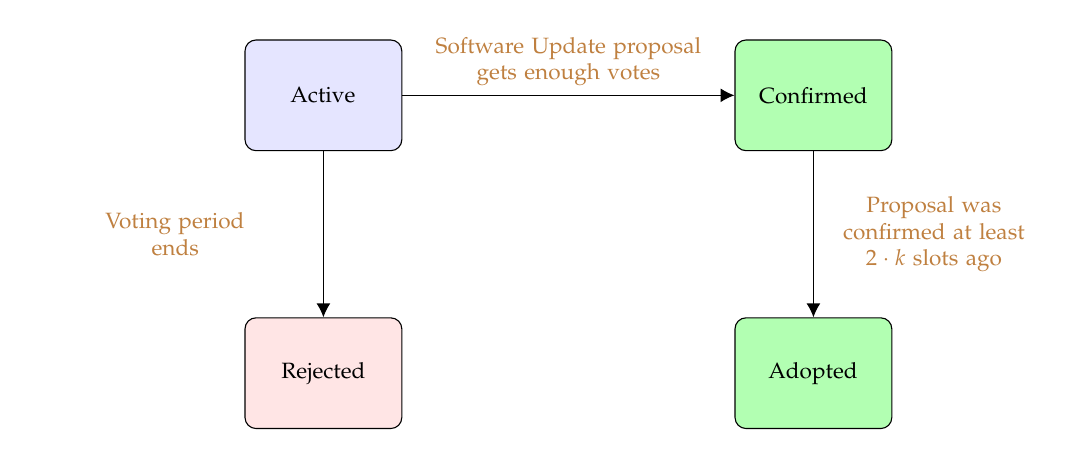
\begin{tikzpicture}[ align = center
                     , node distance = 6em and 12em
                     , text width = 5em
                     , font = \footnotesize
                     , >={Latex[width=0.5em, length=0.5em]}
                     , every node/.style = { rectangle
                                         , rounded corners
                                         , draw = black
                                         , align = center
                                         , minimum height = 4em }
                     ]

  \node (active) [fill = blue!10] {Active};
  \node (rejected) [below = of active, fill = red!10] {Rejected};
  \node (confirmed) [right = of active, fill = green!30] {Confirmed};
  \node (adopted) [below = of confirmed, fill = green!30] {Adopted};

  \tikzset{every node/.style={align=center, text width=10em, text=brown}}

  \draw[->] (active)
  edge node [above] {Software Update proposal\\ gets enough votes}
  (confirmed);

  \draw[->] (active)
  edge node [left] {Voting period \\ends}
  (rejected);

  \draw[->] (confirmed)
  edge node [right, text width=8em]
  {Proposal was confirmed at least $2 \cdot k$ slots ago}
  (adopted);


  \end{tikzpicture}

  \caption{State-transition diagram for software-updates}
  \label{fig:st-diagram-sw-up}
\end{figure}

\clearpage

A sequence of votes can be applied using $\trans{upivotes}{}$ transitions. The
inference rules for them are presented in \cref{fig:rules:upi-votes}.

\begin{figure}[htb]
  \begin{equation}
    \label{eq:rule:upi-votes-base}
    \inference
    {
    }
    {
      {\left(
        \begin{array}{l}
          s_n\\
          \var{dms}
        \end{array}
      \right)}
      \vdash
      \var{us}
      \trans{upivotes}{\epsilon}
      \var{us}
    }
  \end{equation}
  %
  \begin{equation}
    \label{eq:rule:upi-votes-ind}
    \inference
    {
      {\left(
        \begin{array}{l}
          s_n\\
          \var{dms}
        \end{array}
      \right)}
      \vdash
      \var{us}
      \trans{upivotes}{\Gamma}
      \var{us'}
      &
      {\left(
        \begin{array}{l}
          s_n\\
          \var{dms}
        \end{array}
      \right)}
      \vdash
      \var{us'}
      \trans{\hyperref[fig:rules:upi-vote]{upivote}}{v}
      \var{us''}
    }
    {
      {\left(
        \begin{array}{l}
          s_n\\
          \var{dms}
        \end{array}
      \right)}
      \vdash
      \var{us}
      \trans{upivotes}{\Gamma;v}
      \var{us''}
    }
  \end{equation}
  \caption{Applying multiple votes on update-proposals rules}
  \label{fig:rules:upi-votes}
\end{figure}
\clearpage

The interface rule for protocol-version endorsement makes use of the
$\trans{upend}{}$ transition, where we set the threshold for proposal adoption
to: the number of genesis keys ($\var{ngk}$) times the minimum proportion of
genesis keys that need to endorse an update proposal for it to become a
candidate for adoption (given by the protocol parameter $\var{upAdptThd}$). In
addition, the unconfirmed proposals that are older than $u$ blocks are removed
from the parts of the state that hold:
\begin{itemize}
\item the registered protocol and software update proposals,
\item the votes associated with the proposals,
\item the set of endorsement-key pairs, and
\item the block number in which proposals where added.
\end{itemize}

In Rule~\ref{eq:rule:upi-pend}, the set of proposal id's $\var{pid_{keep}}$
contains only those proposals that haven't expired yet or that are confirmed.
Once a proposal $\var{up}$ is confirmed, it is removed from the set of
confirmed proposals ($\var{cps}$) when a new a protocol version gets adopted
(see Rule~\ref{eq:rule:upi-ec-pv-change}).
%
The set of endorsement-key pairs is cleaned here as well as in the epoch change
rule (Rule~\ref{eq:rule:upi-ec-pv-change}). The reason for this is that this set grows at
each block, and it can get considerably large if no proposal gets adopted at
the end of an epoch.

\begin{figure}[htb]
  \begin{equation}
    \label{eq:rule:upi-pend}
    \inference
    {
      \var{upAdptThd} \mapsto q \in \var{pps} \\
      \left({
        \begin{array}{l}
          s_n\\
          \floor{q \cdot \var{ngk}}\\
          \var{dms}\\
          \var{cps}\\
          \var{rpus}
        \end{array}
      }\right)
      \vdash
      {
        \left(
          \begin{array}{l}
            \var{fads}\\
            \var{bvs}
          \end{array}
        \right)
      }
      \trans{\hyperref[fig:rules:up-end]{upend}}{(\var{bv}, \var{vk})}
      {
        \left(
          \begin{array}{l}
            \var{fads'}\\
            \var{bvs'}
          \end{array}
        \right)
      }\\
      \var{upropTTL} \mapsto u \in \var{pps}\\
      {
        \begin{array}{r@{~\leteq~}l}
          \var{pids_{keep}} & \dom~(pws \restrictrange [s_n - u, ..]) \cup \dom~\var{cps}\\
          \var{vs_{keep}} & \dom~(\range~\var{rpus'})\\
          \var{rpus'} & \var{pids_{keep}} \restrictdom \var{rpus}
        \end{array}
      }
    }
    {
      {\left(
        \begin{array}{l}
          s_n\\
          \var{dms}
        \end{array}
      \right)}
      \vdash
      {
        \left(
          \begin{array}{l}
            (\var{pv}, \var{pps})\\
            \var{fads}\\
            \var{avs}\\
            \var{rpus}\\
            \var{raus}\\
            \var{cps}\\
            \var{vts}\\
            \var{bvs}\\
            \var{pws}
          \end{array}
        \right)
      }
      \trans{upiend}{(\var{bv}, \var{vk})}
      {
        \left(
          \begin{array}{l}
            (\var{pv}, \var{pps})\\
            \var{fads'}\\
            \var{avs}\\
            \var{rpus'}\\
            \var{pids_{keep}} \restrictdom \var{raus}\\
            \var{cps}\\
            \var{pids_{keep}} \restrictdom \var{vts}\\
            \var{vs_{keep}}  \restrictdom \var{bvs'}\\
            \var{pids_{keep}} \restrictdom \var{pws}
          \end{array}
        \right)
      }
    }
  \end{equation}
  \caption{Proposal endorsement rules}
  \label{fig:rules:upi-pend}
\end{figure}

\clearpage

Rule~\ref{eq:rule:upi-ec-pv-change} models how the protocol-version and its
parameters are changed depending on an epoch change signal.
%
On an epoch change, this rule will pick a candidate that gathered enough
endorsements at least $2 \cdot k$ slots ago. If a protocol-version candidate
cannot gather enough endorsements $2 \cdot k$ slots before the end of an
epoch, the proposal can only be adopted in the next epoch.
%
Figure~\ref{fig:up-confirmed-too-late} shows an example of a proposal being
confirmed too late in an epoch, where it is not possible to get enough
endorsements in the remaining window. In this Figure we take $k = 2$, and we
assume $4$ endorsements are needed to consider a proposal as candidate for
adoption.
%
Note that, in the final state, we use union override to define the updated
parameters ($\var{pps} \unionoverrideRight \var{pps'}$). This is because candidate
proposal might only update some parameters of the protocol.

In Rule~\ref{eq:rule:upi-ec-pv-change}, when a new proposal gets adopted, all
the state components that refer to protocol update proposals get emptied. The
reason for this is that at the moment of registering a proposal, we evaluated
it in a state where the protocol parameters that we used for this are no longer
up to date (see for instance \cref{eq:func:can-update}). For instance, assume
we register a proposal $\var{up}$ which only changes the maximum transaction
size to $x$, and the current block size is set to $x + 1$. Then,
$\fun{canUpdate}$ holds, since the maximum transaction size is less than the
maximum block size. If now a new proposal gets adopted that changes the maximum
block size to $x - 1$, then this invalidates $\var{up}$ since $\fun{canUpdate}$
no longer holds.
%

If there are no candidates for adoption, then the state variables remain
unaltered (Rule~\ref{eq:rule:upi-ec-pv-unchanged}).

Also note that the registered software-update proposals need not be cleaned
here, since this is done either when a proposal gets confirmed or when it
expires.

\begin{figure}[htb]
  \begin{equation}
    \label{eq:rule:pvbump-change-epoch-only}
    \inference
    {
      [.., s_n - 2 \cdot k] \restrictdom \var{fads} = \epsilon
    }
    {
      {\left(\begin{array}{l}
         s_n\\
         \var{fads}
       \end{array}\right)}
      \vdash
      {
        \left(
          \begin{array}{l}
            \var{pv}, \var{pps}\\
          \end{array}
        \right)
      }
      \trans{pvbump}{}
      {
        \left(
          \begin{array}{l}
            \var{pv}, \var{pps}\\
          \end{array}
        \right)
      }
    }
  \end{equation}
  \nextdef
  \begin{equation}
    \label{eq:rule:pvbump-change}
    \inference
    {
      \wcard ; (\wcard , (\var{pv_c}, \var{pps_c})) \leteq [.., s_n - 2 \cdot k] \restrictdom \var{fads}
    }
    {
      {\left(\begin{array}{l}
         s_n\\
         \var{fads}
       \end{array}\right)}
      \vdash
      {
        \left(
          \begin{array}{l}
            \var{pv}, \var{pps}\\
          \end{array}
        \right)
      }
      \trans{pvbump}{}
      {
        \left(
          \begin{array}{l}
            \var{pv_c}, \var{pps_c}\\
          \end{array}
        \right)
      }
    }
  \end{equation}
  \caption{Protocol version bump rules}
  \label{fig:rules:pvbump}
\end{figure}

\begin{figure}[htb]
  \begin{equation}
    \label{eq:rule:upi-ec-pv-unchanged}
    \inference
    {
      {\left(\begin{array}{l}
         s_n\\
         \var{fads}
       \end{array}\right)}
      \vdash
      {
        \left(
          \begin{array}{l}
            \var{pv}, \var{pps}
          \end{array}
        \right)
      }
      \trans{\hyperref[fig:rules:pvbump]{pvbump}}{}
      {
        \left(
          \begin{array}{l}
            \var{pv'}, \var{pps'}\\
          \end{array}
        \right)
      } &\var{pv} = \var{pv'}
    }
    {
      (s_n)
      \vdash
      {
        \left(
          \begin{array}{l}
            (\var{pv}, \var{pps})\\
            \var{fads}\\
            \var{avs}\\
            \var{rpus}\\
            \var{raus}\\
            \var{cps}\\
            \var{vts}\\
            \var{bvs}\\
            \var{pws}
          \end{array}
        \right)
      }
      \trans{upiec}{}
      {
        \left(
          \begin{array}{l}
            (\var{pv}, \var{pps})\\
            \var{fads}\\
            \var{avs}\\
            \var{rpus}\\
            \var{raus}\\
            \var{cps}\\
            \var{vts}\\
            \var{bvs}\\
            \var{pws}
          \end{array}
        \right)
      }
    }
  \end{equation}
  \nextdef
  \begin{equation}
    \label{eq:rule:upi-ec-pv-change}
    \inference
    {
      {\left(\begin{array}{l}
         s_n\\
         \var{fads}
       \end{array}\right)}
      \vdash
      {
        \left(
          \begin{array}{l}
            \var{pv}, \var{pps}\\
          \end{array}
        \right)
      }
      \trans{\hyperref[fig:rules:pvbump]{pvbump}}{}
      {
        \left(
          \begin{array}{l}
            \var{pv'}, \var{pps'}\\
          \end{array}
        \right)
      }
      & \var{pv} \neq \var{pv'}
    }
    {
      (s_n)
      \vdash
      {
        \left(
          \begin{array}{l}
            \var{(\var{pv}, \var{pps})}\\
            \var{fads}\\
            \var{avs}\\
            \var{rpus}\\
            \var{raus}\\
            \var{cps}\\
            \var{vts}\\
            \var{bvs}\\
            \var{pws}
          \end{array}
        \right)
      }
      \trans{upiec}{}
      {
        \left(
          \begin{array}{l}
            (\var{pv'}, \var{pps'})\\
            \epsilon\\
            \var{avs}\\
            \emptyset\\
            \var{raus}\\
            \emptyset\\
            \emptyset\\
            \emptyset\\
            \emptyset\\
          \end{array}
        \right)
      }
    }
  \end{equation}
  \caption{Block version adoption on epoch change rules}
  \label{fig:rules:upi-ec}
\end{figure}

\begin{figure}[htb]
  \centering
  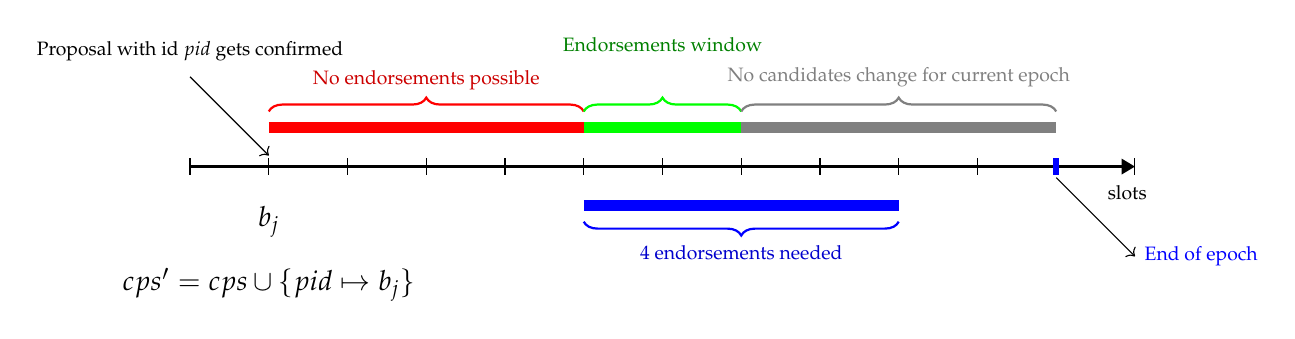
\begin{tikzpicture}
    %%
    %% Macros used in this picture
    %%
    %
    % Number of slots
    \pgfmathsetmacro{\nrSlots}{12}
    % Slot in which the proposal gets confirmed
    \pgfmathsetmacro{\cSlot}{1}
    % Our special K.
    \pgfmathsetmacro{\K}{4}
    % Epoch end.
    \pgfmathsetmacro{\eend}{11}
    % Number of positive votes needed
    \pgfmathsetmacro{\votes}{4}

    % Draw the horizontal line
    \draw[thick, -Triangle] (0,0) -- (\nrSlots,0)
    node[font=\scriptsize,below left=3pt and -8pt]{slots};

    % % draw vertical lines
    \foreach \x in {0,1,...,\nrSlots}
    \draw (\x cm, 3pt) -- (\x cm, -3pt);

    % Add a label to with the block number in which the proposal got confirmed.
    \node at (\cSlot, -.7) {$b_j$};

    % Update in cps
    \node at (\cSlot, -1.5) {$\var{cps'} = \var{cps} \cup \{ \var{pid} \mapsto b_j \}$};

    % The no-endorsements red bar.
    \draw[red, line width=4pt] (\cSlot, .5) -- +(\K, 0);

    % Brace above the no-endorsement window bar.
    \draw[thick, red, decorate, decoration={brace, amplitude=5pt}]
    (\cSlot, .7) -- +(\K, 0)
    node[black!20!red, midway, above=4pt, font=\scriptsize] {No endorsements possible};

    % The endorsements window.
    \coordinate (ewStart) at (\cSlot + \K, .5);
    \coordinate (ewEnd) at ($(\eend - \K, .5)$);
    \draw[green, line width=4pt]
    (ewStart) -- (ewEnd);

    % Brace above the endorsements window
    \coordinate (ewStartB) at ($(ewStart) + (0, 0.2)$);
    \coordinate (ewEndB) at ($(ewEnd) + (0, 0.2)$);
    \draw[thick, green, decorate, decoration={brace, amplitude=5pt}]
    (ewStartB) -- (ewEndB)
    node[black!50!green, midway, above=18pt, font=\scriptsize] {Endorsements window};

    % The no-candidates change window.
    \coordinate (nccStart) at (\eend - \K, .5);
    \coordinate (nccEnd) at ($(\eend, .5)$);
    \draw[gray, line width=4pt]
    (nccStart) -- (nccEnd);

    % Brace above the no-candidates change window.
    \coordinate (nccStartB) at ($(nccStart) + (0, 0.2)$);
    \coordinate (nccEndB) at ($(nccEnd) + (0, 0.2)$);
    \draw[thick, gray, decorate, decoration={brace, amplitude=5pt}]
    (nccStartB) -- (nccEndB)
    node[gray, midway, above=5pt, font=\scriptsize] {No candidates change for current epoch};


    % The 2k before end-of-epoch window.
    \coordinate (beeStart) at (\cSlot + \K, -.5);
    \coordinate (beeEnd) at ($(\cSlot + \K + \votes, -.5)$);
    \draw[blue, line width=4pt]
    (beeStart) -- (beeEnd);

    % Brace on above the 2k before end-of-epoch window.
    \coordinate (beeStartB) at ($(beeStart) - (0, 0.2)$);
    \coordinate (beeEndB) at ($(beeEnd) - (0, 0.2)$);
    \draw[thick, blue, decorate, decoration={brace, amplitude=5pt}]
    (beeEndB) -- (beeStartB)
    node[black!20!blue, midway, below=5pt, font=\scriptsize] {$\votes$ endorsements needed};

    \draw[blue, line width=2pt] (\eend, 3pt) -- (\eend, -3pt);

    \draw[<-] (\cSlot, 4pt) -- +(-1, 1)
    node [above=2pt, black, font=\scriptsize]
    {Proposal with id $\var{pid}$ gets confirmed};

    \draw[->] (\eend, -4pt) -- +(1, -1)
    node[right, blue, font=\scriptsize] {End of epoch};
  \end{tikzpicture}
  \caption{An update proposal confirmed too late}
  \label{fig:up-confirmed-too-late}
\end{figure}

Figure~\ref{fig:st-diagram-pt-up} shows the different states a protocol-update
proposal can be in, and what causes the transitions between them.

\begin{figure}[ht]
  \centering
  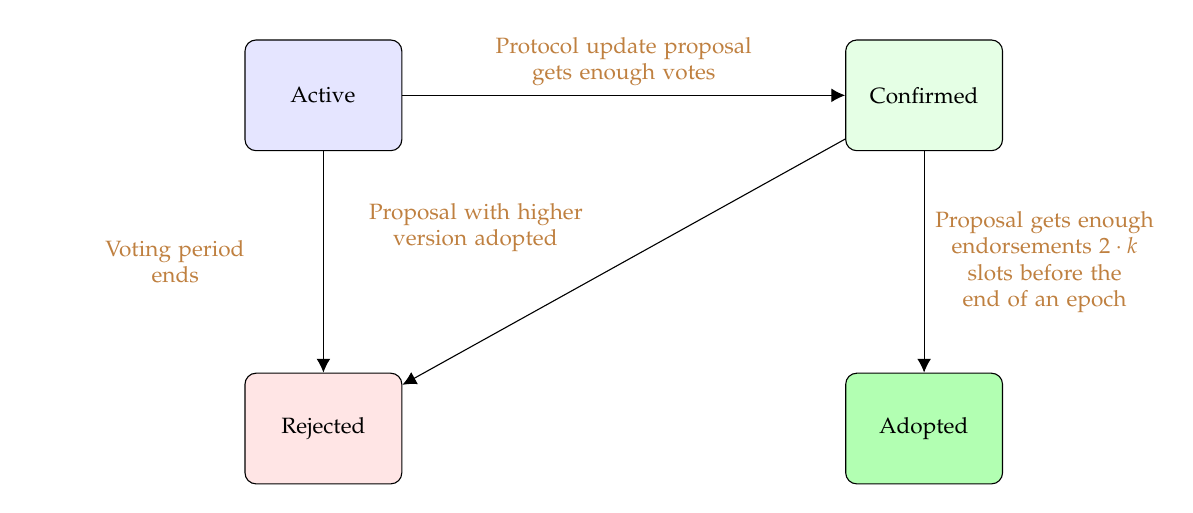
\begin{tikzpicture}[ align = center
                     , node distance = 8em and 16em
                     , text width = 5em
                     , font = \footnotesize
                     , >={Latex[width=0.5em, length=0.5em]}
                     , every node/.style = { rectangle
                                         , rounded corners
                                         , draw = black
                                         , align = center
                                         , minimum height = 4em }
                     ]

  \node (active) [fill = blue!10] {Active};
  \node (rejected) [below = of active, fill = red!10] {Rejected};
  \node (confirmed) [right = of active, fill = green!10] {Confirmed};
  \node (adopted) [below = of confirmed, fill = green!30] {Adopted};

  \tikzset{every node/.style={align=center, text width=10em, text=brown}}

  \draw[->] (active)
  edge node [above] {Protocol update proposal\\ gets enough votes}
  (confirmed);

  \draw[->] (active)
  edge node [left] {Voting period \\ends}
  (rejected);

  \draw[->] (confirmed)
  edge node [above left]
  {Proposal with higher version adopted}
  (rejected);

  \draw[->] (confirmed)
  edge node [right, text width=8em]
  {Proposal gets enough endorsements $2 \cdot k$ slots before the end of an epoch}
  (adopted);

  \end{tikzpicture}

  \caption{State-transition diagram for protocol-updates}
  \label{fig:st-diagram-pt-up}
\end{figure}


In this section we discuss the properties which we want the ledger to have. One
goal is to include these properties in the executable specification for doing
property-based testing or formal verification.

\subsection{Validity of a Ledger State}
\label{sec:valid-ledg-state}

Many properties only make sense when applied to a valid ledger state. In
informal terms, a valid ledger state $l$ can only be reached when starting from
an initial state $l_{0}$ (genesis state) and only executing state transition
rules as specified in Section~\ref{sec:state-trans-utxo-1} for UTxO or
Section~\ref{sec:delegation} for delegation.

\begin{figure}[ht]
  \centering
  \begin{align*}
    \genesisId & \in & \TxId \\
    \genesisTxOut & \in & \TxOut \\
    \genesisUTxO & \coloneqq & \{\genesisId, \emptyset\} \mapsto \genesisTxOut
    \\
    \ledgerState & \in & \left(
                         \begin{array}{c}
                           \UTxO \\
                           \DState \\
                           \PState
                         \end{array}
    \right)\\
               && \\
    \fun{getUTxO} & \in & \ledgerState \to \UTxO \\
    \fun{getUTxO} & \coloneqq & (\var{utxo}, \wcard, \wcard) \to \var{utxo}
  \end{align*}
  \caption{Valid Ledger State}
  \label{fig:valid-ledger}
\end{figure}

In Figure~\ref{fig:valid-ledger} \genesisId{} marks the transaction identifier
of the initial coin distribution, where \genesisTxOut{} represents the initial
UTxO. It should be noted that no corresponding inputs exists, i.e., the
transaction inputs are the empty set for the initial transaction. An element of
\ledgerState{} is a triplet of UTxO, stake delegation state (\DState) and
delegation pool state (\PState).

\begin{definition}[\textbf{Valid Ledger State}]
  \begin{multline*}
    \label{eq:2}
    \forall l_{0},..,l_{n} \in \ledgerState, l_{0} =
    \left(
      \begin{array}{c}
        \left\{
        \genesisUTxO
        \right\} \\
        \emptyset\\
        \emptyset\\
      \end{array}
    \right)  \\
    \implies \forall 0 < i \leq n, ((\exists c \in \DCert, l_{i-1}
    \trans{delegw}{c} l_{i}) \vee (\exists tx \in \Tx: l_{i-1} \trans{utxow}{tx}
    l_{i}))\\ \implies \applyFun{validLedgerState}(l_{n})
  \end{multline*}
  \label{def:valid-ledger-state}
\end{definition}

Definition~\ref{def:valid-ledger-state} defines a valid ledger state reachable
from the genesis state via valid UTxO, stake delegation or stake pool
transactions. This gives a constructive rule how to reach a valid ledger state.

\subsection{Ledger Properties}
\label{sec:ledger-properties}

The following properties state the desired features of updating a valid ledger
state.

\begin{property}[\textbf{Preserve Balance Modulo Fee}]
  \begin{multline*}
    \forall \var{l}, \var{l'} \in \ledgerState: \applyFun{validLedgerstate}{l}\\
    \implies \forall \var{tx} \in \Tx, \var{l} \trans{utxo}{tx} \var{l'}
    \implies \fun{balance}(\applyFun{getUTxO}{l}) =
    \fun{balance}(\applyFun{getUTxO}{l'}) + \applyFun{txfee}{tx}
  \end{multline*}
  \label{prop:ledger-properties-1}
\end{property}

Property~\ref{prop:ledger-properties-1} states that for each valid ledger $l$,
if a transaction $tx$ is added to the ledger via the state transition rule
$utxow$ to the new ledger state $l'$, the balance of the UTxOs in $l$ equals the
balance of the UTxOs in $l'$ minus the transaction fees.

\begin{property}[\textbf{Preserve Balance Restricted to TxIns in Balance of
    TxOuts}]
  \begin{multline*}
    \forall \var{l}, \var{l'} \in \ledgerState: \applyFun{validLedgerstate}{l}\\
    \implies \forall \var{tx} \in \Tx, \var{l} \trans{utxo}{tx} \var{l'}
    \implies \fun{balance}(\applyFun{txins}{tx} \restrictdom
    \applyFun{getUTxO}{l}) = \fun{balance}(\applyFun{txouts}{tx}) +
    \applyFun{txfee}{tx}
  \end{multline*}
  \label{prop:ledger-properties-2}
\end{property}

Property~\ref{prop:ledger-properties-2} states the more detailed relation of the
balances change. For ledgers $l, l'$ and a transaction $tx$ as above, the
balance of the UTxOs of $l$ restricted to those whose domain is in the set of
transaction inputs of $tx$ equals the balance of the transaction outputs of $tx$
minus the transaction fees.

\begin{property}[\textbf{Preserve Outputs of Transaction}]
  \begin{multline*}
    \forall \var{l}, \var{l'} \in \ledgerState: \applyFun{validLedgerstate}{l}\\
    \implies \forall \var{tx} \in \Tx, \var{l} \trans{utxo}{tx} \var{l'}
    \implies \forall \var{out} \in \applyFun{txouts}{tx}, out \in
    \applyFun{getUTxO}{l'}
  \end{multline*}
  \label{prop:ledger-properties-3}
\end{property}

Property~\ref{prop:ledger-properties-3} states that for every ledger states
$l, l'$ and transaction $tx$ as above, all output UTxOs of $tx$ are in the UTxO
set of $l'$, i.e., they are now available as unspent transaction output.

\begin{property}[\textbf{Eliminate Inputs of Transaction}]
  \begin{multline*}
    \forall \var{l}, \var{l'} \in \ledgerState: \applyFun{validLedgerstate}{l}\\
    \implies \forall \var{tx} \in \Tx, \var{l} \trans{utxo}{tx} \var{l'}
    \implies \forall \var{in} \in \applyFun{txins}{tx}, in \not\in
    \fun{dom}(\applyFun{getUTxO}{l'})
  \end{multline*}
  \label{prop:ledger-properties-4}
\end{property}

Property~\ref{prop:ledger-properties-4} states that for every ledger states
$l, l'$ and transaction $tx$ as above, all transaction inputs $in$ of $tx$ are
not in the domain of the UTxO set of $l'$, i.e., these are no longer available
to spend.

\begin{property}[\textbf{Completeness and Collision-Freeness of new Transaction
    Ids}]
  \begin{multline*}
    \forall \var{l}, \var{l'} \in \ledgerState: \applyFun{validLedgerstate}{l}\\
    \implies \forall \var{tx} \in \Tx, \var{l} \trans{utxo}{tx} \var{l'}
    \implies \forall utxo' \in \applyFun{txouts}{tx}, \var{utxo'} \in
    \applyFun{getUTxO}{l'} \wedge \\(\var{utxo'} = ((\var{txId'}, \wcard) \mapsto
    \wcard) \implies \forall \var{utxo} \in \applyFun{getUTxO}{l}, \var{utxo} =
    ((\var{txId}, \wcard) \mapsto \wcard) \implies \var{txId'} \neq \var{txId}
  \end{multline*}
  \label{prop:ledger-properties-5}
\end{property}

Property~\ref{prop:ledger-properties-5} states that for ledger states $l, l'$
and a transaction $tx$ as above, the UTxOs of $l'$ contain all newly created
UTxOs and the referred transaction id of each new UTxO is not used in the UTxO
set of $l$.

%%% Local Variables:
%%% mode: latex
%%% TeX-master: "ledger-spec"
%%% End:


\addcontentsline{toc}{section}{References}
\bibliographystyle{plainnat}
\bibliography{references}

\end{document}
